\documentclass[11pt,letterpaper]{article}
\usepackage{nl_tps_common}
\graphicspath{{figures/}}
\hypersetup{pdftitle={Natural-Language Treatment Planning System Concept of Operations},pdfsubject={NL-TPS controlled documentation}}
\begin{document}
\NLSetPageStyle{NL-TPS CONCEPT OF OPERATIONS}{Natural-Language Treatment Planning System - Version 0.1}
\NLTitleBlock{CONCEPT OF OPERATIONS}{Natural-Language Treatment Planning System}{A human-governed interface for evidence-constrained contouring, disease-site planning, and multi-plan optimization}{\begin{minipage}{0.95\textwidth}
\NLMeta{Version}{0.1 - Discussion Draft}
\NLMeta{Date}{17 August 2026}
\NLMeta{Audience}{Clinical, dosimetry, medical physics, informatics, quality, regulatory, and engineering stakeholders}
\end{minipage}}{This ConOps defines a proposed operating concept. It is not a clinical protocol, commissioning report, regulatory determination, or authorization for patient use.}

\tableofcontents
\clearpage
\pagenumbering{arabic}
\NLFrontMatterSection{Document control}

\begin{small}
\begin{longtable}{@{}L{0.1327\textwidth}L{0.3273\textwidth}L{0.1327\textwidth}L{0.3273\textwidth}@{}}
\toprule
\rowcolor{NLTableHeader}\textbf{\textbf{Field}} & \textbf{\textbf{Value}} & \textbf{\textbf{Field}} & \textbf{\textbf{Value}} \\
\midrule
\endfirsthead
\toprule
\rowcolor{NLTableHeader}\textbf{\textbf{Field}} & \textbf{\textbf{Value}} & \textbf{\textbf{Field}} & \textbf{\textbf{Value}} \\
\midrule
\endhead
\midrule
\multicolumn{4}{r}{\scriptsize Continued on next page} \\
\endfoot
\bottomrule
\endlastfoot
Title & Natural-Language Treatment Planning System - Concept of Operations & Owner & TPS Program Steering Committee (proposed) \\
\addlinespace[2pt]
Version & 0.1 & Status & Discussion Draft - not for clinical use \\
\addlinespace[2pt]
Date & 17 August 2026 & Review cycle & At each design gate and at least annually \\
\addlinespace[2pt]
Primary audience & Radiation oncologists, dosimetrists, medical physicists, therapists, informaticists, quality and regulatory staff, engineers & Scope & External-beam photon and proton planning; research\slash\allowbreak{}training and controlled clinical workflows \\
\end{longtable}
\end{small}

Change history. Version 0.1 establishes the initial operational concept, human authority model, evidence governance, architecture, hazard controls, validation strategy, and staged deployment gates. Future versions should record stakeholder decisions and trace them to requirements, hazards, tests, and approved procedures in accordance with the program's quality system [1-4].

\NLFrontMatterSection{Executive summary}

\begin{nlnotice}{THE OUTCOME WE SEEK}
Create a new, clinically responsible way to practice treatment planning: an authorized user states intent in ordinary language; the system converts that intent into explicit, reviewable planning actions; approved inference and optimization services produce several high-quality candidate plans; and the multidisciplinary team selects, refines, verifies, and approves the plan most appropriate for the patient.
\end{nlnotice}

The proposed Natural-Language Treatment Planning System (NL-TPS) is a command, reasoning, and collaboration layer over validated radiotherapy systems. It is not a replacement for a radiation oncologist, medical dosimetrist, qualified medical physicist, radiation therapist, or established quality management program. It is designed to make clinical intent easier to express, planning alternatives easier to explore, evidence easier to inspect, and every consequential action easier to verify and audit.

The system accepts typed or spoken requests such as: 'Create three robust proton candidates for this approved head-and-neck intent, preserve target coverage, and explore different swallowing-structure tradeoffs.' It does not execute that sentence directly. It binds the active patient and dataset, converts the request to a typed plan-intent object, identifies ambiguity, retrieves institution-approved and cited evidence, previews the actions and assumptions, obtains required confirmations, and invokes commissioned contouring, optimization, and dose-calculation services. The output is a set of clinical candidates with provenance, uncertainties, constraint status, and role-specific review views.

The central safety idea is separation of powers. Generative or inference models may interpret language, retrieve evidence, suggest contours, propose objectives, and orchestrate reversible sandbox actions. They may not prescribe, sign, approve, release, or deliver treatment. Dose is calculated by commissioned engines within their validated use envelope. Independent checks use a separate method, data path, or responsible owner. Human sign-off remains mandatory at the clinical transitions defined in this ConOps [29-39].

\subsection{The program in one page}

\begin{itemize}
\item \textbf{Clinical mission.} Improve the quality, diversity, traceability, and efficiency of planning while preserving professional judgment and independent safety controls.
\item \textbf{Primary users.} Radiation oncologists, medical dosimetrists, qualified medical physicists, and radiation therapists, supported by informatics, quality, regulatory, cybersecurity, and engineering teams.
\item \textbf{Core capabilities.} Natural-language plan intent, evidence-constrained disease-site support, AI-assisted contour drafting, multi-objective candidate generation, transparent plan comparison, structured refinement, and complete provenance.
\item \textbf{Initial scope.} External-beam photon and proton planning using CT and approved adjunct imaging. Brachytherapy, radiopharmaceutical therapy, autonomous adaptive delivery, and direct machine control are outside the initial clinical scope.
\item \textbf{Operating modes.} Training\slash\allowbreak{}research, commissioning, shadow, clinical draft, approved clinical, and degraded\slash\allowbreak{}read-only modes are physically and logically separated.
\item \textbf{Evidence constraint.} Clinical recommendations and constraints must originate from a governed evidence library containing patient orders, trial protocols, institutional standards, professional guidance, and curated literature with version and applicability metadata.
\item \textbf{Success standard.} Demonstrate that the human-AI team is at least as safe as the current process, produces clinically acceptable and meaningfully diverse plans, preserves independent verification, improves planning effort or cycle time, and detects its own limitations.
\end{itemize}

\section{Purpose, audience, and ConOps status}

This ConOps communicates what the NL-TPS is intended to accomplish, who will use it, how work will flow, where authority will reside, what external systems and evidence it will depend on, and how the program will demonstrate readiness. Its structure follows the intent of ISO\slash\allowbreak{}IEC\slash\allowbreak{}IEEE 29148 for stakeholder-oriented operational concepts and is meant to precede detailed system, software, interface, data, and clinical requirements [1].

The document serves four purposes: align the clinical and engineering vision; make safety boundaries testable; expose policy and workflow decisions that require governance; and provide a basis for requirements, risk management, human-factors work, regulatory strategy, procurement, validation, and staged implementation.

\subsection{In scope}

\begin{itemize}
\item Text and speech interaction for trained, authenticated professional users.
\item Patient-context acquisition; image and structure review; rigid or deformable registration only through commissioned tools and approved workflows.
\item Disease-site and planning-template assistance grounded in verified patient facts and approved evidence.
\item AI-assisted OAR and target contour drafting, uncertainty display, edit capture, and approval workflows.
\item Plan-goal authoring, conflict detection, multi-objective optimization, robust proton planning, photon planning, dose calculation, and candidate comparison through commissioned services.
\item Interoperability with DICOM RT, RT Ion objects, current IHE-RO profiles, ROIS\slash\allowbreak{}TPS systems, and EHR data interfaces where supported [23-28].
\item Clinical governance, audit, model\slash\allowbreak{}evidence lifecycle management, cybersecurity, downtime, training, monitoring, and incident learning.
\item A separate training mode using synthetic or de-identified cases for education, rehearsal, and competency assessment.
\end{itemize}

\subsection{Out of scope for the first clinical release}

\begin{itemize}
\item Autonomous diagnosis, staging, prescription, final contour approval, plan approval, treatment authorization, or radiation delivery.
\item Background-listening voice control, unattended case processing, or execution of ambiguous free-form instructions.
\item Uncontrolled self-learning, online weight updates, or automatic replacement of clinical models or evidence.
\item Brachytherapy, radiopharmaceutical therapy, total-body\slash\allowbreak{}total-skin techniques, and other special procedures unless separately scoped and commissioned.
\item Outcome claims based only on dosimetric surrogates. Candidate plans can expose tradeoffs; they do not prove a superior patient outcome without appropriate clinical evidence.
\item Substitution for independent dose\slash\allowbreak{}MU verification, patient-specific QA, physics plan review, peer review, or required institutional checklists [33-39].
\end{itemize}

\section{Operational need and future-state vision}

\subsection{Current-state problem}

Modern treatment planning distributes one clinical intent across many interfaces, documents, naming conventions, optimization objectives, machine models, and review steps. Users repeatedly translate between clinical language and system-specific commands. Constraints may be copied without their original population, fractionation, endpoint, dose basis, or version. Plans are often optimized serially, so the team sees only a small portion of the feasible trade space. Automation can reduce keystrokes while still increasing risk if it obscures assumptions, weakens independent review, or encourages automation bias.

Proton planning adds sensitivity to range, setup, anatomy, motion, material assignment, beam angle, and robustness assumptions. A natural-language interface is valuable only if it makes those assumptions more explicit, not less. AAPM and IAEA guidance consistently place treatment planning within an institutional QA program involving acceptance, commissioning, ongoing QA, data-transfer checks, role-appropriate review, and risk-based workflow analysis [29-43,56].

\subsection{Future-state experience}

In the future state, the planner begins with a verified patient context and an approved physician planning directive. The user can speak or type at the level of clinical intent. The interface compiles that intent into a structured, unit-aware, modality-aware representation. It shows what it understood, the evidence and institutional protocol it proposes to apply, missing information, assumptions, and the actions that will occur. The user can revise the structured intent directly or in natural language.

Once confirmed, the system can prepare contours, objectives, and several candidate plans in a sandbox. It reports feasibility, hard-constraint violations, sensitivity and robustness, model limitations, and clinically interpretable tradeoffs rather than collapsing everything into an unexplained score. The radiation oncologist, dosimetrist, and physicist review the same plan objects through lenses appropriate to their responsibilities. Their edits, overrides, comments, and approvals remain attributable. The chosen plan then follows conventional independent QA, transfer, and treatment-release controls.

\subsection{Program goals and measurable intent}

\begin{small}
\begin{longtable}{@{}L{0.1769\textwidth}L{0.3715\textwidth}L{0.3715\textwidth}@{}}
\toprule
\rowcolor{NLTableHeader}\textbf{\textbf{Goal}} & \textbf{\textbf{Operational meaning}} & \textbf{\textbf{Evidence of success}} \\
\midrule
\endfirsthead
\toprule
\rowcolor{NLTableHeader}\textbf{\textbf{Goal}} & \textbf{\textbf{Operational meaning}} & \textbf{\textbf{Evidence of success}} \\
\midrule
\endhead
\midrule
\multicolumn{3}{r}{\scriptsize Continued on next page} \\
\endfoot
\bottomrule
\endlastfoot
G1 - Safe expression of intent & Convert ordinary language into explicit, typed, unit-aware actions with read-back and risk-based confirmation. & No clinically consequential action occurs from unresolved or unconfirmed intent. \\
\addlinespace[2pt]
G2 - Evidence-grounded planning & Attach source, version, applicability, and local approval to every proposed clinical objective or constraint. & Users can trace each active rule to the governing order, protocol, or approved source. \\
\addlinespace[2pt]
G3 - Better exploration & Generate clinically feasible, robust, deliverable, and meaningfully different candidate plans. & The team sees distinct tradeoffs, not cosmetic variations of one solution. \\
\addlinespace[2pt]
G4 - Preserved authority & Keep prescription, contour, physics, plan, and release decisions with qualified professionals. & Electronic gates enforce role and separation-of-duties rules. \\
\addlinespace[2pt]
G5 - Reproducibility & Record data, models, algorithms, machine configuration, evidence, prompts\slash\allowbreak{}intent, parameters, seeds, and edits. & A released candidate can be reconstructed or its differences explained. \\
\addlinespace[2pt]
G6 - Sustainable learning & Monitor performance, drift, near misses, overrides, subgroup effects, and workflow outcomes. & Changes enter production only through approved validation and rollback-ready release control. \\
\end{longtable}
\end{small}

\section{Guiding principles and non-negotiable boundaries}

\begin{itemize}
\item \textbf{Human accountability is indivisible.} The system may assist a role but may not impersonate that role's professional judgment or signature.
\item \textbf{Natural language is an input method, not a safety specification.} Every consequential request must become a typed command with explicit objects, units, scope, and preconditions.
\item \textbf{Grounding is necessary but not sufficient.} A citation does not guarantee applicability. Population, disease site, laterality, modality, dose basis, fractionation, endpoint, and institutional approval must match.
\item \textbf{Calculation is separate from generation.} Language and generative models do not calculate clinical dose. Commissioned dose engines and machine models do.
\item \textbf{Independent checks remain independent.} The verification path must not silently reuse the same model, corrupted source data, assumptions, or code path as the primary calculation.
\item \textbf{Uncertainty must be visible and actionable.} The interface should surface model applicability, image quality, registration concerns, contour uncertainty, robustness assumptions, and unsupported requests.
\item \textbf{Reversibility precedes commitment.} AI actions occur in a sandbox and produce a preview\slash\allowbreak{}diff before they alter a clinical object or cross a system boundary.
\item \textbf{No silent failure and no silent fallback.} The system clearly enters a degraded state, stops unsafe work, preserves the ledger, and directs users to the approved manual workflow.
\item \textbf{Local commissioning governs local use.} Vendor validation, publication performance, or another institution's results cannot replace site-specific acceptance and clinical commissioning [30,39-43].
\item \textbf{Patient benefit governs optimization.} Efficiency and dosimetric metrics are means, not the final objective. Claims about outcomes require clinical validation and surveillance.
\end{itemize}

\begin{nlnotice}{PROHIBITED CLINICAL ACTIONS}
The NL-TPS will not autonomously create or modify a signed prescription, approve target volumes, approve a treatment plan, release a plan to treatment, waive independent QA, or command a treatment delivery system.
\end{nlnotice}

\section{Stakeholders, authority, and responsibility}

The system is designed around a multidisciplinary team, not a single 'AI user.' Roles may be adapted to local credentials and policy, but authority boundaries must remain explicit. ASTRO's safety framework and APEx standards describe radiation oncology as a coordinated process with written directives, documented prescriptions, plan evaluation, signatures, QA, information-system controls, and a comprehensive quality program [53-54].

\begin{small}
\begin{longtable}{@{}L{0.1474\textwidth}L{0.4777\textwidth}L{0.2949\textwidth}@{}}
\toprule
\rowcolor{NLTableHeader}\textbf{\textbf{Stakeholder}} & \textbf{\textbf{Operational responsibility}} & \textbf{\textbf{Authority boundary}} \\
\midrule
\endfirsthead
\toprule
\rowcolor{NLTableHeader}\textbf{\textbf{Stakeholder}} & \textbf{\textbf{Operational responsibility}} & \textbf{\textbf{Authority boundary}} \\
\midrule
\endhead
\midrule
\multicolumn{3}{r}{\scriptsize Continued on next page} \\
\endfoot
\bottomrule
\endlastfoot
Patient & Source of preferences, values, consent, and relevant history through the clinical team; not an NL-TPS operator in the initial release. & No direct planning authority. \\
\addlinespace[2pt]
Radiation oncologist & Defines clinical intent, target concepts, prescription, tradeoff priorities, and clinical acceptability; approves target contours and final plan. & Accountable for prescription and clinical plan approval. \\
\addlinespace[2pt]
Medical dosimetrist & Builds and refines planning strategies; evaluates geometry and dosimetry; edits AI output; documents planning decisions. & Accountable for planning work within assigned scope; cannot self-authorize physician or physics gates. \\
\addlinespace[2pt]
Qualified medical physicist & Commissions systems and models; defines validated use envelopes; reviews algorithms, robustness, deliverability, calculations, data transfer, and QA. & Accountable for technical commissioning, physics review, and independent verification program. \\
\addlinespace[2pt]
Radiation therapist & Contributes simulation, immobilization, setup, imaging, and delivery-operability knowledge; verifies treatment instructions and delivery context. & Accountable for assigned simulation\slash\allowbreak{}delivery checks; cannot release an unapproved plan. \\
\addlinespace[2pt]
Clinical informatics \slash\allowbreak{} IT \slash\allowbreak{} cybersecurity & Operates interfaces, identity, infrastructure, backups, monitoring, access, incident response, and downtime processes. & Accountable for service operation, not clinical decisions. \\
\addlinespace[2pt]
Quality \slash\allowbreak{} safety \slash\allowbreak{} regulatory & Maintains QMS, risk files, CAPA, document control, human-factors evidence, regulatory strategy, complaint and incident processes. & Accountable for governance evidence and escalation. \\
\addlinespace[2pt]
AI \slash\allowbreak{} software \slash\allowbreak{} data engineering & Develops and maintains software and models under change control; supplies verification evidence and limitations. & No clinical approval authority; no direct production changes. \\
\addlinespace[2pt]
Clinical governance committee & Approves intended use, evidence sources, protocols, risk acceptance, model releases, monitoring thresholds, and clinical expansion. & Final institutional authority for deployment scope. \\
\end{longtable}
\end{small}

\subsection{Separation of duties}

\begin{itemize}
\item The person or service that generates a candidate cannot satisfy all approval and independent-check requirements for that candidate.
\item A user may hold more than one credentialed role, but the system records the role exercised at each action and enforces local policy for independent review.
\item Model owners may not approve their own model for clinical release without independent validation and governance review.
\item Evidence curators may propose updates; clinical owners approve applicability and effective dates.
\end{itemize}

\section{Operating modes and autonomy envelope}

Mode is a safety property, not a visual theme. Data, credentials, interfaces, model permissions, output labeling, and audit behavior must prevent a research or training object from becoming a clinical object without an approved transition.

\begin{small}
\begin{longtable}{@{}L{0.1474\textwidth}L{0.3833\textwidth}L{0.3892\textwidth}@{}}
\toprule
\rowcolor{NLTableHeader}\textbf{\textbf{Mode}} & \textbf{\textbf{Permitted work}} & \textbf{\textbf{Required isolation \slash\allowbreak{} controls}} \\
\midrule
\endfirsthead
\toprule
\rowcolor{NLTableHeader}\textbf{\textbf{Mode}} & \textbf{\textbf{Permitted work}} & \textbf{\textbf{Required isolation \slash\allowbreak{} controls}} \\
\midrule
\endhead
\midrule
\multicolumn{3}{r}{\scriptsize Continued on next page} \\
\endfoot
\bottomrule
\endlastfoot
Training \slash\allowbreak{} research & Synthetic, public, or appropriately de-identified cases; exploratory models and prompts permitted. & No clinical destinations; persistent watermark\slash\allowbreak{}label; separate tenancy and keys. \\
\addlinespace[2pt]
Commissioning & Golden cases, phantom data, retrospective cohorts, challenge cases, workflow tests, and human-factors studies. & Clinical-like configuration but no treatment release; controlled evidence capture. \\
\addlinespace[2pt]
Shadow & Processes current clinical cases in parallel without influencing care. & Outputs hidden from treating team unless protocol permits; prospective performance collection. \\
\addlinespace[2pt]
Clinical draft & Creates reviewable contours, objectives, and candidate plans inside the planning workspace. & All outputs are unsigned drafts; confirmation and role gates enforced. \\
\addlinespace[2pt]
Clinical approved & Contains human-approved objects eligible for established QA and controlled export. & Objects become immutable or versioned; changes invalidate downstream approvals. \\
\addlinespace[2pt]
Degraded \slash\allowbreak{} read-only & Allows retrieval of completed work and audit records during partial service failure. & No new clinical execution; explicit downtime procedure and reconciliation. \\
\end{longtable}
\end{small}

\subsection{Autonomy levels}

\begin{small}
\begin{longtable}{@{}L{0.1622\textwidth}L{0.3833\textwidth}L{0.3745\textwidth}@{}}
\toprule
\rowcolor{NLTableHeader}\textbf{\textbf{Level}} & \textbf{\textbf{Example}} & \textbf{\textbf{Control}} \\
\midrule
\endfirsthead
\toprule
\rowcolor{NLTableHeader}\textbf{\textbf{Level}} & \textbf{\textbf{Example}} & \textbf{\textbf{Control}} \\
\midrule
\endhead
\midrule
\multicolumn{3}{r}{\scriptsize Continued on next page} \\
\endfoot
\bottomrule
\endlastfoot
A0 - Inform & Search, explain, display, compare, cite. & May run immediately after patient\slash\allowbreak{}context checks; no mutation. \\
\addlinespace[2pt]
A1 - Draft & Prepare a proposed note, contour set, objective set, checklist, or plan request. & User review required before the draft enters the clinical workspace. \\
\addlinespace[2pt]
A2 - Sandbox execute & Run reversible transformations, contour inference, optimization, or dose calculation in a draft workspace. & Structured preview, explicit confirmation, complete ledger, cancel\slash\allowbreak{}rollback. \\
\addlinespace[2pt]
A3 - Clinical candidate & Promote a validated draft to a named clinical candidate. & Role-based review and signatures; no release to treatment. \\
\addlinespace[2pt]
A4 - Authorize or deliver & Approve prescription\slash\allowbreak{}plan, waive QA, release or command delivery. & Prohibited for AI; performed only by authorized humans and established systems. \\
\end{longtable}
\end{small}

\section{Operational concept and end-to-end workflow}

\begin{figure}[htbp]
\centering
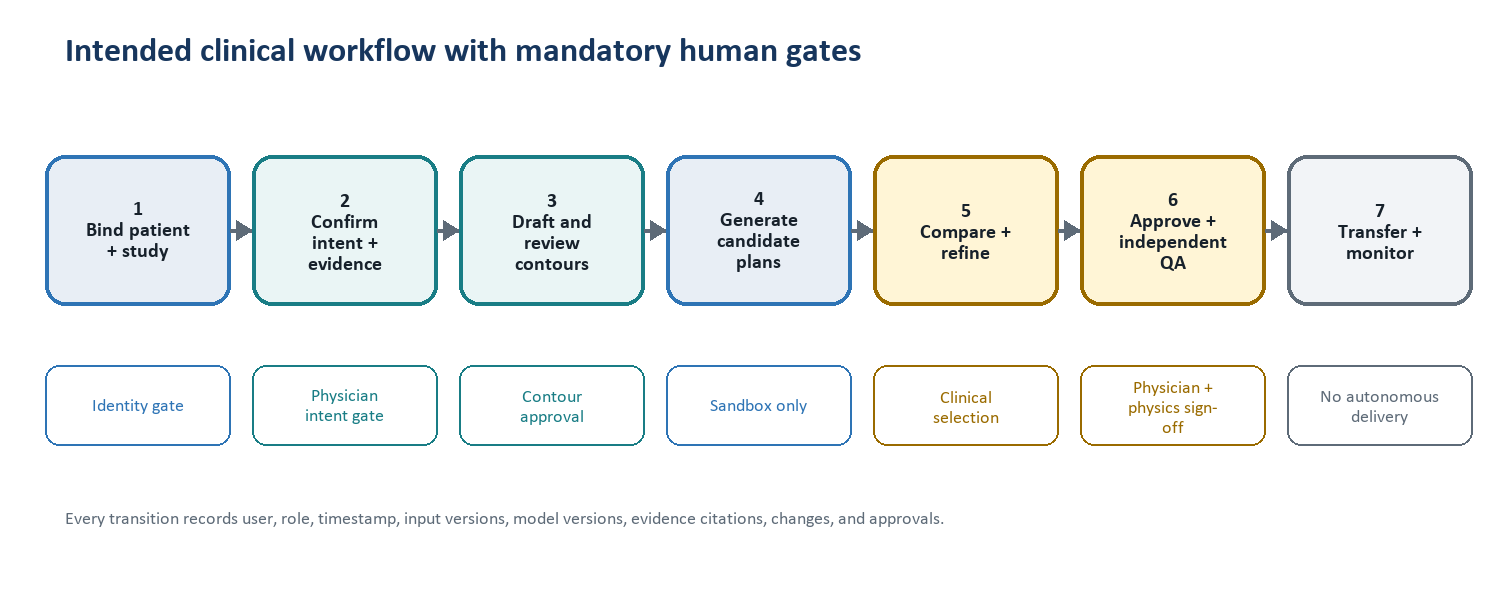
\includegraphics[width=0.96\textwidth]{clinical-workflow.png}
\caption{Intended clinical workflow. AI activity remains inside the governed draft path until human approval and independent QA are complete.}
\label{fig:clinical-workflow}
\end{figure}

\begin{enumerate}
\item \textbf{Establish patient, course, and dataset context.} The user selects the patient and course from the source system. The NL-TPS displays at least two patient identifiers, encounter\slash\allowbreak{}course, planning study UID, acquisition date, frame of reference, modality, orientation, and prior-plan context. The user confirms the active context before any mutation.
\item \textbf{Compile clinical intent.} The system imports the signed planning directive\slash\allowbreak{}prescription when available and extracts disease site, laterality, targets, dose\slash\allowbreak{}fractionation, technique\slash\allowbreak{}modality, image guidance, prior radiation, special risks, and tradeoff priorities. It distinguishes verified facts from inferred or missing fields.
\item \textbf{Select and validate the evidence package.} The system proposes the applicable institutional protocol, trial protocol, professional guidance, and toxicity literature. It checks version, population, modality, fractionation, dose basis, structure definitions, and conflicts. A clinical owner confirms the package.
\item \textbf{Prepare images, registrations, and contours.} Commissioned registration and segmentation services create drafts with model\slash\allowbreak{}applicability metadata. Users review overlays and uncertainty indicators, edit contours, and approve according to role. Target approval remains a physician action.
\item \textbf{Create the structured plan intent.} The user states goals in clinical language. The compiler produces a machine-readable intent containing hard constraints, optimization objectives, priority relationships, robustness scenarios, allowed techniques, machine, algorithm, and candidate diversity request.
\item \textbf{Generate and calculate candidate plans.} The orchestrator submits explicit jobs to approved planning and dose engines. Each plan remains within the commissioned envelope and receives immutable provenance. Infeasible or unsupported requests stop with a clear explanation.
\item \textbf{Compare and refine.} The workspace presents target coverage, OAR dose, hotspots, dose bath, robustness, complexity, deliverability, uncertainty, and evidence compliance. It shows deltas between candidates and the effect of requested changes. Users can ask for refinements; each request creates a new version.
\item \textbf{Approve, verify, and transfer.} The selected plan receives clinical approval, physics review, independent dose\slash\allowbreak{}MU verification and\slash\allowbreak{}or patient-specific QA as required, checklist completion, and validated data transfer. Any downstream-changing edit invalidates the affected approvals.
\item \textbf{Monitor and learn.} The system records execution health, overrides, failures, drift signals, QA outcomes, near misses, and user corrections. Governance reviews these signals without using patient data for retraining unless an approved protocol and data governance process permit it.
\end{enumerate}

\section{Primary clinical use cases}

\subsection{Disease-site and intent assistant}

The assistant helps organize known information; it does not silently diagnose. It may map a documented diagnosis, anatomic site, pathology, stage, prior treatment, and physician directive to a candidate disease-site template. It must show which facts are source-verified, which are user-entered, and which remain unknown. A disease-site suggestion becomes active only after confirmation by an authorized clinician.

\begin{itemize}
\item Retrieve the current institution-approved planning template and supporting guidance for the confirmed disease site and treatment context.
\item Identify missing or conflicting facts that materially affect contouring, modality, fractionation, margins, constraints, or technique.
\item Summarize the exact source and rationale for each proposed planning rule; never cite a source that the evidence service did not retrieve and verify.
\item Escalate reirradiation, pediatric, pregnancy, implanted-device, motion, altered anatomy, unusual fractionation, and clinical-trial cases to specialized workflows.
\end{itemize}

\subsection{AI-assisted contouring}

A contour model produces a draft RT Structure Set or segmentation object for the intended image series. The system displays structure name mapping, model version, intended population and modality, input quality checks, uncertainty or anomaly indicators, and comparison with institutional contouring conventions. TG-132 principles govern registrations; TG-263 governs naming; evolving AAPM work on clinical implementation of AI segmentation is monitored but is not treated as published normative guidance until finalized [32,35,45].

\begin{itemize}
\item OAR contours may be reviewed and approved by staff authorized under institutional policy; target contours require radiation oncologist approval.
\item The interface must support slice, surface, and clinically relevant error review, not only a global similarity metric.
\item Every edit is recorded. Large or patterned edits trigger a model-performance review signal rather than being treated only as user preference.
\item Low-confidence, out-of-distribution, truncated anatomy, artifact, contrast mismatch, postoperative change, and registration-dependent contours stop or route to manual review.
\end{itemize}

\subsection{Multi-plan generation and comparison}

The system generates a configurable set of candidates that are both clinically acceptable and meaningfully diverse. Diversity may involve beam arrangement, modality, robustness strategy, OAR tradeoff, dose falloff, integral dose, or complexity - but never a change to the signed prescription or an unapproved clinical assumption. For protons, candidate generation explicitly captures setup and range uncertainty, density overrides, motion\slash\allowbreak{}interplay strategy, beam-specific targets when used, and robustness evaluation consistent with the commissioned workflow [40-43,48].

The comparison view does not crown a universal 'best plan.' It first separates feasible from infeasible plans, then presents hard-constraint status and clinically interpretable tradeoffs. Role-specific views emphasize: disease control and toxicity for the physician; plan construction and refinement for the dosimetrist; and calculation validity, robustness, complexity, deliverability, transfer, and QA for the physicist. The team can record why a plan was selected and why alternatives were rejected.

\subsection{Adaptive and replanning workflow}

Adaptive use is a later release with a separate safety case. It requires a new image-quality and registration assessment, verified structure propagation or recontouring, dose accumulation assumptions, change detection, a new plan-intent version, and reapproval of all affected objects. IEC 62083:2025 includes adaptive radiotherapy within the safety scope of a TPS, and TG-132 emphasizes that registration output becomes input to planning or delivery and therefore requires understood uncertainty and QA [2,32].

\section{Natural-language interaction contract}

The conversational interface is useful because it lets professionals communicate at the level of intent. It is safe only when the system treats language as fallible. Every request passes through the sequence below before execution.

\begin{small}
\begin{longtable}{@{}L{0.1474\textwidth}L{0.7726\textwidth}@{}}
\toprule
\rowcolor{NLTableHeader}\textbf{\textbf{Stage}} & \textbf{\textbf{Required behavior}} \\
\midrule
\endfirsthead
\toprule
\rowcolor{NLTableHeader}\textbf{\textbf{Stage}} & \textbf{\textbf{Required behavior}} \\
\midrule
\endhead
\midrule
\multicolumn{2}{r}{\scriptsize Continued on next page} \\
\endfoot
\bottomrule
\endlastfoot
1. Capture & Record typed text or a user-confirmed speech transcript. Voice uses push-to-talk; background listening and voice-only signatures are prohibited. \\
\addlinespace[2pt]
2. Bind context & Attach the request to the active patient, course, study, plan version, role, and mode. If context is missing or changed, stop. \\
\addlinespace[2pt]
3. Compile & Translate language into a typed intent schema with objects, actions, parameters, units, priorities, evidence references, preconditions, and expected outputs. \\
\addlinespace[2pt]
4. Validate & Check permissions, clinical state, structure names, units, dose basis, machine\slash\allowbreak{}model availability, evidence applicability, and commissioned use envelope. \\
\addlinespace[2pt]
5. Resolve ambiguity & Ask for missing information when an assumption could change dose, anatomy, modality, fractionation, robustness, or approval status. Benign defaults may be used only when documented and previewed. \\
\addlinespace[2pt]
6. Read back & Display a concise, structured preview: what will change, which plan\slash\allowbreak{}object, evidence and assumptions, expected runtime, and how to cancel or roll back. \\
\addlinespace[2pt]
7. Confirm & Apply risk-based confirmation and, where policy requires, a second role or signature. \\
\addlinespace[2pt]
8. Execute and verify & Run the typed command, validate outputs, compare them with the preview, and keep them in draft state. \\
\addlinespace[2pt]
9. Record & Write the immutable command ledger, model\slash\allowbreak{}evidence versions, result hashes, warnings, user edits, approvals, and downstream transfers. \\
\end{longtable}
\end{small}

\subsection{Ambiguity and high-risk triggers}

\begin{itemize}
\item Laterality, target\slash\allowbreak{}structure identity, course or phase, current versus prior study, dose unit, physical versus RBE-weighted dose, relative versus absolute dose, fractionation, maximum versus near-maximum dose, structure volume definition, hard versus soft priority, machine, modality, technique, uncertainty scenario, or normalization method is absent or inconsistent.
\item The request references 'standard,' 'usual,' 'better,' 'spare,' 'maximize,' or 'robust' without a selected institutional definition.
\item A voice transcript contains low-confidence words, negation, numbers, units, drug names, structure names, or laterality.
\item The request conflicts with the signed prescription, trial protocol, approved contour state, evidence package, commissioned machine model, or role permission.
\item The requested transformation would invalidate an approval, transfer, QA result, or treatment record.
\end{itemize}

\subsection{Illustrative interaction}

\begin{nlnotice}{USER}
'Make three proton plans. Keep the target coverage the same, improve oral cavity and swallowing dose, and show me the robustness tradeoff.'
\end{nlnotice}

\begin{nlnotice}{SYSTEM READ-BACK}
'Active case: [two identifiers], approved planning CT [date\slash\allowbreak{}UID], plan-intent version 4. I will create three draft PBS candidates using the commissioned machine and dose engine, the approved prescription, the confirmed head-and-neck protocol, and the current range\slash\allowbreak{}setup scenarios. Target coverage will remain a hard goal. Oral cavity and swallowing structures will be varied as soft priorities. No approved object will change. Confirm candidate count, machine, and robustness package.'
\end{nlnotice}

\begin{nlnotice}{SAFETY RESPONSE}
If the prescription, approved target set, dose basis, structure identity, or robustness package is missing or inconsistent, the system stops and identifies the exact unresolved field instead of guessing.
\end{nlnotice}

\section{Evidence-constrained reasoning and literature governance}

The evidence service is a controlled clinical knowledge base, not an unrestricted web search. It stores approved documents and computable rules with provenance and change control. The clinical system may retrieve only sources admitted by governance for the relevant jurisdiction and intended use. External search can support curation in a nonclinical workflow, but it cannot silently introduce a new rule into patient planning.

\subsection{Operational precedence and conflict handling}

\begin{small}
\begin{longtable}{@{}L{0.1769\textwidth}L{0.4335\textwidth}L{0.3096\textwidth}@{}}
\toprule
\rowcolor{NLTableHeader}\textbf{\textbf{Operational tier}} & \textbf{\textbf{Examples}} & \textbf{\textbf{Use rule}} \\
\midrule
\endfirsthead
\toprule
\rowcolor{NLTableHeader}\textbf{\textbf{Operational tier}} & \textbf{\textbf{Examples}} & \textbf{\textbf{Use rule}} \\
\midrule
\endhead
\midrule
\multicolumn{3}{r}{\scriptsize Continued on next page} \\
\endfoot
\bottomrule
\endlastfoot
Patient-specific authority & Signed prescription\slash\allowbreak{}directive, physician-approved intent, informed decisions, prior-treatment facts. & Highest case-specific authority; discrepancies stop work. \\
\addlinespace[2pt]
Protocol authority & Enrolled clinical-trial protocol, credentialing requirements, approved protocol amendments. & Applied exactly for enrolled cases; conflicts are escalated, not blended. \\
\addlinespace[2pt]
Institutional standard & Approved disease-site templates, contouring atlases, machine\slash\allowbreak{}technique policies, action levels. & Default local practice with owner and effective date. \\
\addlinespace[2pt]
Professional guidance & AAPM MPPGs\slash\allowbreak{}TG reports, ASTRO\slash\allowbreak{}ACR\slash\allowbreak{}ESTRO guidance, ICRU, IAEA, QUANTEC\slash\allowbreak{}HyTEC\slash\allowbreak{}PENTEC, NRG\slash\allowbreak{}cooperative-group material when applicable. & Supports institutional rules; applicability and currency must be reviewed [29-56]. \\
\addlinespace[2pt]
Peer-reviewed evidence & Systematic reviews, trials, validated datasets, individual studies. & May support curation or research; not automatically promoted to a clinical constraint. \\
\end{longtable}
\end{small}

This ordering is an operational conflict policy, not a grading of scientific evidence. A new safety warning or guideline can require immediate suspension of an older local template. The evidence governance committee owns exception, retirement, and escalation rules.

\subsection{Minimum metadata for a computable planning rule}

\begin{itemize}
\item Canonical rule ID; human-readable statement; original source title, version\slash\allowbreak{}date, section\slash\allowbreak{}table\slash\allowbreak{}page, and licensed access reference.
\item Institutional owner, approval status, effective date, review date, superseded\slash\allowbreak{}retired status, and linked change record.
\item Disease site, intent, population, age group, laterality, organ\slash\allowbreak{}target definition, treatment technique, modality, and image\slash\allowbreak{}contour prerequisites.
\item Dose quantity and basis: physical absorbed dose, RBE-weighted dose, BED\slash\allowbreak{}EQD2 only when explicitly supported; fractionation, alpha\slash\allowbreak{}beta assumption when relevant, volume metric, endpoint, time horizon, and uncertainty.
\item Rule type: prescription, hard limit, planning goal, optimization objective, reporting metric, caution, or contraindication.
\item Applicability logic, exclusions, evidence strength\slash\allowbreak{}limitations, conflict policy, and required human approver.
\item Machine-readable units, comparator, tolerance, structure nomenclature mapping, test examples, and validation status.
\end{itemize}

\subsection{Literature baseline}

The initial governed corpus should include current local protocols plus selected primary sources. ICRU reports define common concepts for prescribing, recording, and reporting photon and proton therapy. QUANTEC summarizes conventional-fractionation normal-tissue dose-volume evidence; HyTEC addresses high-dose-per-fraction treatment; PENTEC addresses pediatric normal-tissue effects. These sources have known limitations and cannot be reduced to universal hard limits without clinical interpretation [46-51]. ASTRO disease-site guidelines and current cooperative-group protocols can inform clinical intent, while AAPM and IAEA documents govern physics, planning, and QA practice [29-44,52-56].

\begin{nlnotice}{DOSE-CONSTRAINT SAFETY}
The system must never copy a dose limit without its source, population, contour definition, endpoint, dose basis, and fractionation context. It must not convert between physical dose, RBE-weighted dose, BED, or EQD2 unless an approved, visible method and assumptions are selected.
\end{nlnotice}

\section{System context and logical architecture}

\begin{figure}[htbp]
\centering
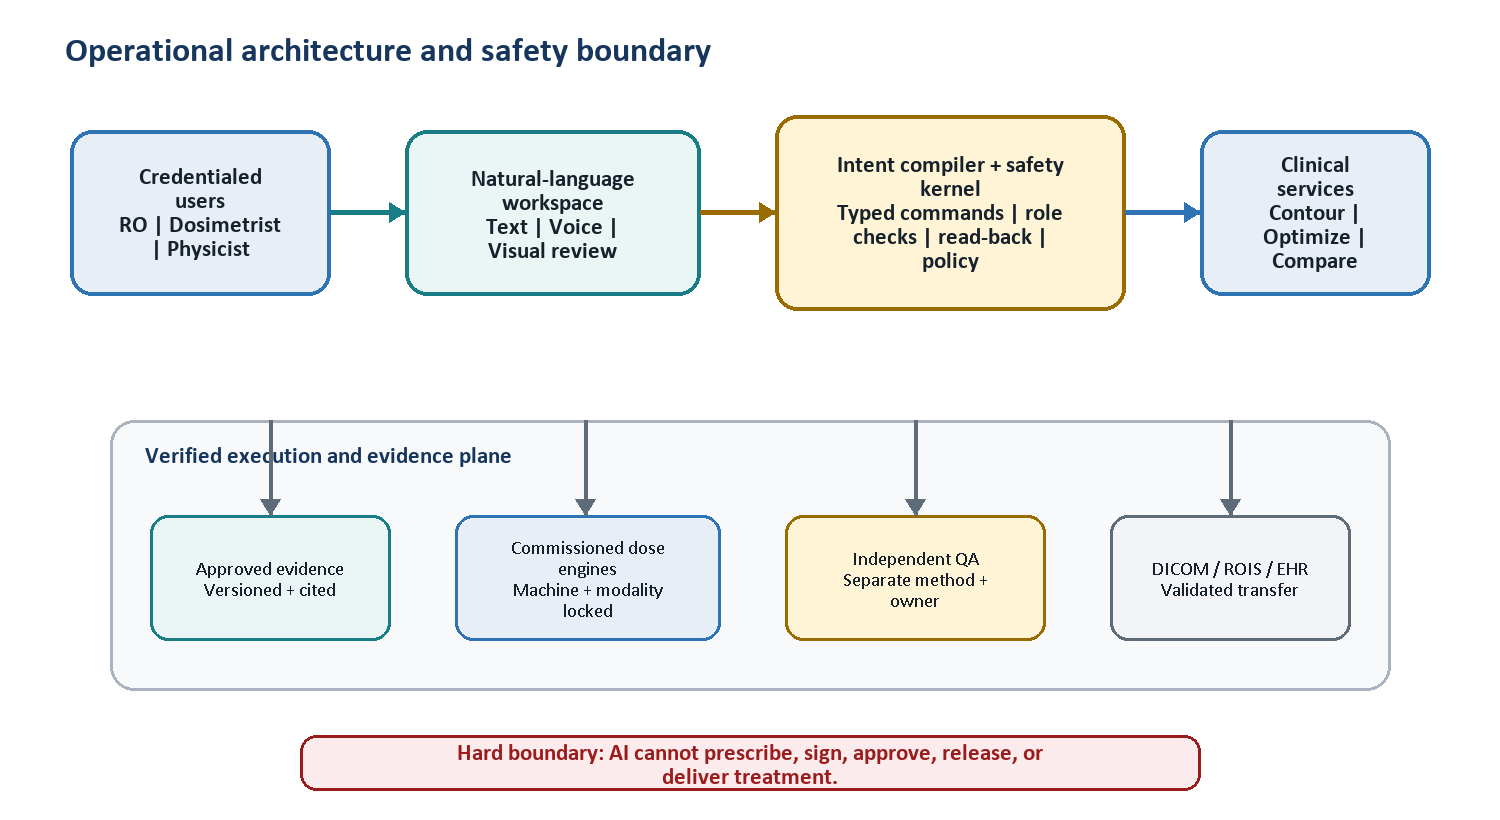
\includegraphics[width=0.96\textwidth]{logical-architecture.png}
\caption{Logical architecture. The safety kernel and verified execution plane prevent free-form language from directly controlling a clinical plan or treatment system.}
\label{fig:logical-architecture}
\end{figure}

\begin{small}
\begin{longtable}{@{}L{0.2064\textwidth}L{0.7136\textwidth}@{}}
\toprule
\rowcolor{NLTableHeader}\textbf{\textbf{Component}} & \textbf{\textbf{Operational responsibility}} \\
\midrule
\endfirsthead
\toprule
\rowcolor{NLTableHeader}\textbf{\textbf{Component}} & \textbf{\textbf{Operational responsibility}} \\
\midrule
\endhead
\midrule
\multicolumn{2}{r}{\scriptsize Continued on next page} \\
\endfoot
\bottomrule
\endlastfoot
Identity and context manager & Authenticates the user and role; binds patient, course, study, frame of reference, plan version, mode, and destination; prevents cross-patient or cross-mode actions. \\
\addlinespace[2pt]
Conversation workspace & Text\slash\allowbreak{}voice input, transcript confirmation, structured read-back, command preview, warnings, citations, plan comparison, visual diffs, and approval surfaces. \\
\addlinespace[2pt]
Intent compiler & Transforms language into a versioned plan-intent schema; separates facts, user preferences, evidence-derived rules, assumptions, and unresolved questions. \\
\addlinespace[2pt]
Clinical safety kernel & Applies role permissions, state machine, patient\slash\allowbreak{}context assertions, commissioned-use checks, hard stops, confirmation level, approval invalidation, and export policy. It is deterministic and independently testable. \\
\addlinespace[2pt]
Evidence service & Retrieves versioned, approved clinical knowledge and emits cited, applicability-checked rules. It does not use unrestricted internet content in clinical mode. \\
\addlinespace[2pt]
Model gateway & Routes to approved segmentation, classification, prediction, and language models; enforces model version, input contract, intended population, resource limits, logging, and out-of-distribution response. \\
\addlinespace[2pt]
Clinical planning services & Image registration, contour drafting, objective creation, optimization, robustness analysis, commissioned dose calculation, and plan evaluation through vendor-neutral adapters where feasible. \\
\addlinespace[2pt]
Candidate and trade-space service & Maintains plan lineage, feasibility, constraint status, diversity, Pareto relationships, robustness, complexity, deliverability, and role-specific comparison views. \\
\addlinespace[2pt]
Independent verification service & Receives a controlled data package through a separate path; performs independent dose\slash\allowbreak{}MU or other QA; does not share hidden state with the primary engine. \\
\addlinespace[2pt]
Interoperability gateway & Validates DICOM, RT Plan, RT Ion Plan, RT Dose, structures\slash\allowbreak{}segmentations, registration, treatment records, IHE-RO transactions, and FHIR-based course\slash\allowbreak{}phase\slash\allowbreak{}plan summaries where implemented [23-28]. \\
\addlinespace[2pt]
Provenance and audit ledger & Stores immutable event records, object hashes, source UIDs, model\slash\allowbreak{}evidence\slash\allowbreak{}software\slash\allowbreak{}configuration versions, structured intent, changes, warnings, approvals, exports, and reconciliation. \\
\addlinespace[2pt]
Monitoring and governance console & Tracks safety, performance, drift, fairness, reliability, cybersecurity, incidents, evidence currency, model status, and change-control gates. \\
\end{longtable}
\end{small}

\subsection{Interoperability position}

\begin{itemize}
\item Use the current DICOM standard and published conformance statements. Support first-generation RT objects required by installed systems and a deliberate migration path to second-generation RT objects; preserve SOP Instance UIDs, frame-of-reference integrity, derivation, and version lineage [23-25].
\item Conform to applicable IHE-RO profiles rather than claiming generic 'DICOM compatibility.' Current profiles include Basic RT Objects, multimodality registration, treatment planning content, delivery workflow, and ion treatment records [26].
\item Use HL7 FHIR R4 and the CodeX Radiation Therapy implementation guide where appropriate for prescriptions, planned courses\slash\allowbreak{}phases\slash\allowbreak{}plans, treated plans, and summaries; do not use FHIR as a substitute for geometric DICOM content [27].
\item Maintain coordinate-system consistency with IEC 61217 and validate every transformation between image, planning, and delivery coordinate frames [28].
\end{itemize}

\section{Core information and provenance model}

The plan-intent object is the central contract between the human conversation and deterministic clinical services. It must be inspectable without reading a model's hidden reasoning. A minimum object model includes the entities below.

\begin{small}
\begin{longtable}{@{}L{0.1769\textwidth}L{0.7431\textwidth}@{}}
\toprule
\rowcolor{NLTableHeader}\textbf{\textbf{Entity}} & \textbf{\textbf{Minimum content}} \\
\midrule
\endfirsthead
\toprule
\rowcolor{NLTableHeader}\textbf{\textbf{Entity}} & \textbf{\textbf{Minimum content}} \\
\midrule
\endhead
\midrule
\multicolumn{2}{r}{\scriptsize Continued on next page} \\
\endfoot
\bottomrule
\endlastfoot
Case context & Patient identifiers, course\slash\allowbreak{}phase, encounter, diagnosis facts, prior RT, active study and frame, user\slash\allowbreak{}role, mode. \\
\addlinespace[2pt]
Prescription intent & Targets, dose, fractionation, technique\slash\allowbreak{}modality, energy or beam type, normalization, imaging, schedule, author\slash\allowbreak{}signature, status. \\
\addlinespace[2pt]
Anatomy set & Images, registrations, structures, approvals, naming map, segmentation model and edits, structure lineage. \\
\addlinespace[2pt]
Evidence package & Selected protocols, rules, applicability, citations, versions, conflicts, approvals, effective dates. \\
\addlinespace[2pt]
Planning strategy & Machine, beam geometry constraints, objectives, hard\slash\allowbreak{}soft priorities, robustness scenarios, motion strategy, algorithm\slash\allowbreak{}grid\slash\allowbreak{}model. \\
\addlinespace[2pt]
Candidate plan & Unique ID\slash\allowbreak{}version, parent intent, parameters, dose, DVHs, robustness results, complexity, warnings, model\slash\allowbreak{}engine configuration, status. \\
\addlinespace[2pt]
Review and decision & Comparisons, comments, deviations, rationale, role-specific checks, approvals, invalidations, selected\slash\allowbreak{}rejected status. \\
\addlinespace[2pt]
QA and transfer & Independent calculation, measurement\slash\allowbreak{}log QA where required, data-transfer verification, destination, treatment record linkage. \\
\addlinespace[2pt]
Operational evidence & Command ledger, timing, errors, overrides, edits, drift flags, security events, incident\slash\allowbreak{}CAPA linkage. \\
\end{longtable}
\end{small}

\subsection{Data integrity rules}

\begin{itemize}
\item Clinical objects are immutable after approval. A change creates a new version and automatically invalidates affected downstream approvals and QA evidence.
\item Every derived object references its inputs, transformation, software\slash\allowbreak{}model configuration, user or service identity, timestamp, and reason.
\item The system prevents patient merges, study relinking, frame changes, or structure substitutions from occurring as conversational side effects.
\item Units are explicit and validated at storage and interface boundaries. Display rounding never changes calculation values.
\item Clinical retention, legal record status, and export to the official RO-EMR are defined by institutional policy and TG-262-informed practices [38].
\end{itemize}

\section{AI and inference model strategy}

The program may use different model classes for different tasks. A single foundation model should not become an unbounded clinical authority. Each model is treated as a controlled component with an intended use, input\slash\allowbreak{}output contract, model card, data documentation, validation evidence, limitations, owner, version, monitoring plan, and retirement criteria. FDA\slash\allowbreak{}IMDRF good machine learning practice emphasizes multidisciplinary expertise, representative and independent datasets, the performance of the human-AI team, clear user information, monitoring, and managed retraining [11-12,16-17].

\begin{small}
\begin{longtable}{@{}L{0.1622\textwidth}L{0.4099\textwidth}L{0.3479\textwidth}@{}}
\toprule
\rowcolor{NLTableHeader}\textbf{\textbf{Model class}} & \textbf{\textbf{Permitted contribution}} & \textbf{\textbf{Clinical boundary}} \\
\midrule
\endfirsthead
\toprule
\rowcolor{NLTableHeader}\textbf{\textbf{Model class}} & \textbf{\textbf{Permitted contribution}} & \textbf{\textbf{Clinical boundary}} \\
\midrule
\endhead
\midrule
\multicolumn{3}{r}{\scriptsize Continued on next page} \\
\endfoot
\bottomrule
\endlastfoot
Language \slash\allowbreak{} speech & Transcription, intent compilation, summarization, clarification, evidence retrieval, explanation. & No numerical dose calculation or authority; exact numbers\slash\allowbreak{}units\slash\allowbreak{}laterality require deterministic validation and read-back. \\
\addlinespace[2pt]
Disease-site mapping & Map verified clinical facts to candidate workflow\slash\allowbreak{}template and detect missing information. & No autonomous diagnosis or staging; clinician confirmation required. \\
\addlinespace[2pt]
Segmentation & Draft OAR or target contours for supported anatomy and imaging. & Site-specific validation, uncertainty\slash\allowbreak{}anomaly behavior, human review and approval. \\
\addlinespace[2pt]
Planning \slash\allowbreak{} optimization & Warm starts, objective tuning, beam candidates, knowledge-based planning, Pareto sampling. & Outputs must be recalculated and evaluated by commissioned engines; use envelope and reproducibility controlled. \\
\addlinespace[2pt]
Prediction \slash\allowbreak{} outcome & Optional research estimates of toxicity, control, or plan quality. & Not a clinical outcome claim unless independently validated for intended population and use; limitations visible [44,49-51]. \\
\addlinespace[2pt]
QA anomaly detection & Flag unusual contours, parameters, dose, transfer, or workflow patterns. & Augments but does not replace required checks; false-negative risk explicitly assessed. \\
\end{longtable}
\end{small}

\subsection{Model lifecycle controls}

\begin{itemize}
\item Clinical models are locked. No production learning occurs from user edits or patient outcomes. Retraining is an offline, approved change with independent validation and release control.
\item Development, tuning, internal testing, external testing, and site-acceptance datasets are separated and protected from leakage. Cohort composition and relevant demographic, scanner, disease-site, and technique subgroups are reported.
\item Performance is evaluated at the model, task, workflow, and human-team levels. Average performance cannot conceal unacceptable subgroup or rare-hazard behavior.
\item The model must abstain or route to manual review when inputs are unsupported, corrupted, incomplete, out of distribution, or outside the commissioned envelope.
\item Model and dependency supply chains are inventoried; artifacts are signed, scanned, reproducibly built where practicable, and rollback-ready.
\item A change to model weights, prompt templates that alter clinical behavior, retrieval corpus, post-processing, dose engine, machine model, or safety rule is configuration-controlled and impact-assessed.
\end{itemize}

\section{Safety engineering and preliminary hazard analysis}

Safety management combines ISO 14971 lifecycle risk management with the process-oriented failure analysis advocated by AAPM TG-100. The program must maintain a living hazard analysis, process maps, FMEA\slash\allowbreak{}fault-tree work where useful, risk-control traceability, verification evidence, residual-risk decisions, and production feedback [4,31]. The table below is a starting point, not a substitute for institution-specific analysis.

\begin{small}
\begin{longtable}{@{}L{0.0639\textwidth}L{0.3244\textwidth}L{0.5318\textwidth}@{}}
\toprule
\rowcolor{NLTableHeader}\textbf{\textbf{ID}} & \textbf{\textbf{Hazard and potential harm}} & \textbf{\textbf{Required control strategy}} \\
\midrule
\endfirsthead
\toprule
\rowcolor{NLTableHeader}\textbf{\textbf{ID}} & \textbf{\textbf{Hazard and potential harm}} & \textbf{\textbf{Required control strategy}} \\
\midrule
\endhead
\midrule
\multicolumn{3}{r}{\scriptsize Continued on next page} \\
\endfoot
\bottomrule
\endlastfoot
H-01 & Wrong patient, course, study, frame of reference, or plan version; could result in planning for the wrong anatomy or prescription. & Two identifiers; source-system launch context; UID\slash\allowbreak{}frame checks; persistent patient banner; context confirmation; cross-patient action block; immutable linkage; simulation of wrong-context cases. \\
\addlinespace[2pt]
H-02 & Speech\slash\allowbreak{}NLP error, negation failure, number\slash\allowbreak{}unit error, laterality error, or ambiguous instruction. & Push-to-talk; transcript confirmation; typed intent; deterministic unit\slash\allowbreak{}laterality parser; high-risk ambiguity list; structured read-back; no voice signature; test accents\slash\allowbreak{}noise\slash\allowbreak{}interruptions. \\
\addlinespace[2pt]
H-03 & Hallucinated, outdated, or inapplicable clinical recommendation or dose constraint. & Closed evidence service; exact citation\slash\allowbreak{}version\slash\allowbreak{}location; applicability metadata; conflict detection; no-source\slash\allowbreak{}no-rule behavior; curator approval; emergency retirement; user-accessible limitations. \\
\addlinespace[2pt]
H-04 & Prescription, trial protocol, or physician intent is altered or overridden. & Signed-source import; immutable prescription; difference check; role restrictions; hard stop on conflict; new signature after change. \\
\addlinespace[2pt]
H-05 & Contour is missing, mislabeled, geometrically implausible, truncated, or clinically wrong. & TG-263 naming; input\slash\allowbreak{}OOD checks; structure completeness and topology rules; visual uncertainty; slice\slash\allowbreak{}surface review; edit capture; physician target approval; independent review for high-risk structures. \\
\addlinespace[2pt]
H-06 & Rigid\slash\allowbreak{}deformable registration is unsuitable and propagates incorrect anatomy or dose. & Commissioned registration; TG-132 workflow; fusion visualization; quantitative\slash\allowbreak{}qualitative QA; uncertainty statement; registration-specific approval; stop unsupported dose accumulation. \\
\addlinespace[2pt]
H-07 & Dose basis, RBE, fractionation, BED\slash\allowbreak{}EQD2, or structure definition is mismatched. & Explicit quantity model; unit-safe schema; approved conversion methods only; show assumptions; source applicability checks; proton-specific labels; hard stop on ambiguity. \\
\addlinespace[2pt]
H-08 & Dose calculation or machine model is used outside its commissioned envelope. & Machine\slash\allowbreak{}algorithm\slash\allowbreak{}model lock; allowed-technique matrix; MPPG 5.b and proton commissioning tests; runtime configuration attestation; reference-case QA; physics-owned release [30,40-43]. \\
\addlinespace[2pt]
H-09 & Proton range\slash\allowbreak{}setup\slash\allowbreak{}motion\slash\allowbreak{}interplay uncertainty is omitted or misconfigured. & Approved scenario package; required robustness fields; site-specific motion SOP; scenario-completeness test; robust evaluation before candidate eligibility; physics review. \\
\addlinespace[2pt]
H-10 & Candidate plans appear diverse but share a hidden systematic defect or are infeasible\slash\allowbreak{}undeliverable. & Feasibility gate; diversity metrics; independent recalculation; complexity\slash\allowbreak{}deliverability rules; shared-input hazard analysis; alternative method or manual baseline; no winner by opaque composite score. \\
\addlinespace[2pt]
H-11 & Optimization silently relaxes a hard constraint or changes clinical priority. & Typed hard\slash\allowbreak{}soft semantics; immutable constraint set per run; explicit relaxation request and reason; pre\slash\allowbreak{}post diff; violated-hard-constraint block. \\
\addlinespace[2pt]
H-12 & DICOM or other data transfer corrupts, omits, transforms, or associates plan data incorrectly. & Conformance validation; UID\slash\allowbreak{}reference\slash\allowbreak{}coordinate checks; source-destination comparison; TG-201\slash\allowbreak{}TG-262-informed transfer QA; checksum\slash\allowbreak{}hash; reject partial transfer; end-to-end testing. \\
\addlinespace[2pt]
H-13 & AI output weakens independent review through shared logic, data, or automation bias. & Document independence claims; separate QA path\slash\allowbreak{}owner; blinded or staged review where appropriate; display raw clinical evidence; require active checks; monitor override and miss patterns [34,36-39]. \\
\addlinespace[2pt]
H-14 & Unauthorized access, prompt injection, malicious document, model compromise, or PHI leakage. & Least privilege\slash\allowbreak{}MFA; network segmentation; signed evidence; input sanitization; no external tools in clinical mode; encryption; egress control; secure development\slash\allowbreak{}SBOM; logging; tested incident response [7,13,20-22]. \\
\addlinespace[2pt]
H-15 & Stale evidence\slash\allowbreak{}model, drift, subgroup failure, or performance degradation is not detected. & Version registry; expiry\slash\allowbreak{}review date; sentinel cases; subgroup dashboards; edit\slash\allowbreak{}override\slash\allowbreak{}QA monitoring; alert thresholds; kill switch; rollback; periodic revalidation; CAPA. \\
\addlinespace[2pt]
H-16 & Partial outage or timeout leaves an incomplete plan that appears valid. & Atomic job states; visible progress; fail-closed promotion; draft watermark; reconciliation; idempotent retry; downtime plan; no silent fallback; recovery testing. \\
\addlinespace[2pt]
H-17 & A post-approval edit invalidates contours, dose, QA, or transfer without detection. & Dependency graph; immutable versions; automatic approval invalidation; delta review; re-run affected checks; destination reconciliation. \\
\addlinespace[2pt]
H-18 & Users over-trust fluent explanations or under-trust valid alerts. & Human-factors design; calibrated limitations; citations and evidence preview; no anthropomorphic authority cues; scenario-based training; summative validation; monitoring of alert burden and workarounds [5,14-15,17]. \\
\end{longtable}
\end{small}

\begin{nlnotice}{SAFETY CASE}
Clinical release requires an evidence-backed argument that each unacceptable risk is controlled, each control is verified in the integrated workflow, residual risk is reviewed by authorized governance, and monitoring can detect when the argument no longer holds.
\end{nlnotice}

\section{Verification, validation, commissioning, and clinical evaluation}

Validation is layered because correctness at one layer cannot establish safe clinical performance. A fluent conversation can compile to the wrong action; a geometrically accurate contour can still be clinically unacceptable; a high-quality dose distribution can still be calculated with the wrong patient, prescription, or machine. The program therefore verifies requirements, software, data, models, integrations, dose and geometry, workflow, human factors, and post-deployment performance.

\begin{small}
\begin{longtable}{@{}L{0.1710\textwidth}L{0.3981\textwidth}L{0.3509\textwidth}@{}}
\toprule
\rowcolor{NLTableHeader}\textbf{\textbf{Layer}} & \textbf{\textbf{Question}} & \textbf{\textbf{Representative evidence}} \\
\midrule
\endfirsthead
\toprule
\rowcolor{NLTableHeader}\textbf{\textbf{Layer}} & \textbf{\textbf{Question}} & \textbf{\textbf{Representative evidence}} \\
\midrule
\endhead
\midrule
\multicolumn{3}{r}{\scriptsize Continued on next page} \\
\endfoot
\bottomrule
\endlastfoot
Requirements and risk controls & Trace each stakeholder need and hazard control to design, implementation, test, result, anomaly, and release decision. & Requirements trace matrix; risk-control verification report; unresolved anomaly disposition. \\
\addlinespace[2pt]
Language and intent & Test semantic accuracy, numbers\slash\allowbreak{}units, negation, laterality, context, ambiguity, unsafe\slash\allowbreak{}adversarial requests, accents and noise, confirmation, and reproducibility. & Gold utterance corpus; scenario tests; human review; safety-stop sensitivity and false-alert analysis. \\
\addlinespace[2pt]
Evidence service & Verify source identity, version, citation location, applicability, conflict logic, rule computation, retirement, and no-source behavior. & Curated test pack; independent clinical review; regression suite; evidence change audit. \\
\addlinespace[2pt]
Segmentation & Evaluate technical geometry, organ\slash\allowbreak{}site-specific acceptability, dose impact, edit burden, failure detection, subgroup performance, and human-team effect. & Locked external\slash\allowbreak{}site test cohorts; expert review; edit\slash\allowbreak{}time study; uncertainty\slash\allowbreak{}OOD challenge cases. \\
\addlinespace[2pt]
Planning and dose & Commission algorithms, machine models, optimizers, robustness, biological models if used, DVH\slash\allowbreak{}evaluation, and numerical reproducibility for supported techniques. & MPPG 5.b\slash\allowbreak{}TG-53\slash\allowbreak{}proton commissioning evidence; reference plans; measurements; independent calculations [29-44]. \\
\addlinespace[2pt]
Interoperability & Test DICOM\slash\allowbreak{}IHE\slash\allowbreak{}FHIR conformance, geometry, UIDs, structure mapping, plan\slash\allowbreak{}record content, partial\slash\allowbreak{}failure cases, and source-to-destination fidelity. & Conformance statements; connectathon\slash\allowbreak{}vendor tests; end-to-end clinical data-transfer validation. \\
\addlinespace[2pt]
Workflow and human factors & Evaluate representative users, tasks, environments, time pressure, interruptions, handoffs, warnings, approvals, recovery, and critical use errors. & Formative studies; simulated-use and summative validation; training\slash\allowbreak{}competency evidence [5,14-15]. \\
\addlinespace[2pt]
Clinical evaluation & Demonstrate safety, plan acceptability, diversity, efficiency, and human-team performance in retrospective, shadow, and controlled prospective stages. & Predefined endpoints; independent adjudication; protocol\slash\allowbreak{}IRB\slash\allowbreak{}regulatory pathway as applicable. \\
\addlinespace[2pt]
Production monitoring & Detect reliability, drift, subgroup degradation, unsafe overrides, incidents, cybersecurity issues, and evidence\slash\allowbreak{}model obsolescence. & Dashboards; alert\slash\allowbreak{}action thresholds; periodic review; CAPA and rollback exercises. \\
\end{longtable}
\end{small}

\subsection{Model- and workflow-specific metrics}

\begin{itemize}
\item Contouring: structure presence and labeling; Dice only as one descriptor; surface\slash\allowbreak{}95th-percentile Hausdorff or surface distance; clinically significant boundary errors; dose impact; correction time; added path length\slash\allowbreak{}edit burden; case-level failure; reviewer acceptability; OOD sensitivity; subgroup results.
\item Disease-site support: verified-fact extraction, missing-data detection, guideline\slash\allowbreak{}template concordance, citation correctness, applicability errors, conflict escalation, and rate of inappropriate confident recommendations.
\item Planning: feasible-plan rate, target coverage, OAR metrics, hotspots\slash\allowbreak{}coldspots, conformity\slash\allowbreak{}dose falloff, integral dose, robustness worst-case and distributional behavior, plan complexity, deliverability, independent-check results, QA outcomes, diversity, time to first feasible plan, refinement effort, and expert preference with rationale.
\item Natural language: intent exact match by safety-critical slot, numerical\slash\allowbreak{}unit\slash\allowbreak{}laterality error, clarification rate, unsafe execution rate, false stop rate, transcript correction, action-preview comprehension, and task completion under representative interruptions.
\item Human-AI team: clinically important errors, catches, time, workload, interprofessional communication, trust calibration, automation bias, workaround frequency, override appropriateness, and competency retention.
\end{itemize}

\subsection{Commissioning principles}

\begin{itemize}
\item Commission the installed configuration, not a generic product. Include scanners, protocols, image characteristics, network interfaces, TPS\slash\allowbreak{}ROIS versions, machine and dose models, local structure names, clinical protocols, and user roles.
\item Use representative normal cases, boundary cases, rare but foreseeable hazards, corrupted\slash\allowbreak{}partial inputs, prior-treatment cases, pediatric and reirradiation cases when in scope, and deliberately unsafe commands.
\item Create immutable golden cases and reference outputs for regression. Where nondeterminism is allowed, define acceptable distributions and reproducibility controls rather than expecting bitwise identity.
\item Perform end-to-end tests from source images and orders through plan generation, approval invalidation, QA package, transfer, destination comparison, downtime, and recovery.
\item Document the validated use envelope. Unsupported cases are blocked or clearly routed to the approved conventional workflow.
\end{itemize}

\section{Human factors, usability, and training}

The interface changes how users perceive state, interpret evidence, and act on the planning system. It is therefore a safety-critical user interface, not merely a convenience feature. IEC 62366-1 and current FDA human-factors guidance require a risk-based process focused on intended users, use environments, critical tasks, use errors, risk controls, and validation [5,14-15].

\subsection{Human-factors requirements}

\begin{itemize}
\item The active patient, plan, study, mode, approval state, and unsaved\slash\allowbreak{}unverified changes remain continuously visible.
\item The system distinguishes verified patient facts, signed clinical intent, evidence-derived rules, AI suggestions, user entries, and assumptions using consistent visual and textual cues.
\item Warnings identify the hazard and required action. They do not rely on color alone and do not offer a reflexive 'OK' path for high-risk conditions.
\item Plan comparisons show absolute values, deltas, uncertainty\slash\allowbreak{}robustness, violated constraints, and spatial dose - not only rankings or a composite score.
\item Confirmation burden is proportional to risk. Repetitive low-value alerts are measured and redesigned because alert fatigue is itself a hazard.
\item Critical tasks are tested with radiation oncologists, dosimetrists, physicists, and therapists in representative workflows, displays, noise, interruptions, time pressure, and handoffs.
\item Accessibility includes keyboard operation, readable contrast and typography, non-color cues, clear focus state, and alternatives to speech. Speech is optional, not required for clinical function.
\end{itemize}

\subsection{Training and competency}

\begin{small}
\begin{longtable}{@{}L{0.2064\textwidth}L{0.7136\textwidth}@{}}
\toprule
\rowcolor{NLTableHeader}\textbf{\textbf{Audience}} & \textbf{\textbf{Competency focus}} \\
\midrule
\endfirsthead
\toprule
\rowcolor{NLTableHeader}\textbf{\textbf{Audience}} & \textbf{\textbf{Competency focus}} \\
\midrule
\endhead
\midrule
\multicolumn{2}{r}{\scriptsize Continued on next page} \\
\endfoot
\bottomrule
\endlastfoot
All clinical users & System purpose and limits; patient\slash\allowbreak{}context checks; evidence labels; command preview; uncertainty; downtime; incident reporting; avoiding automation bias. \\
\addlinespace[2pt]
Radiation oncologists & Intent\slash\allowbreak{}prescription authority, target approval, clinical tradeoff review, guideline applicability, overrides and rationale. \\
\addlinespace[2pt]
Dosimetrists & Intent editing, contour review, optimization strategy, candidate diversity, feasibility, refinement, and plan lineage. \\
\addlinespace[2pt]
Medical physicists & Commissioning, machine\slash\allowbreak{}dose model controls, robustness, independent QA, data transfer, model\slash\allowbreak{}evidence change assessment, kill switch. \\
\addlinespace[2pt]
Therapists & Simulation and setup data, delivery-context review, treatment instructions, transfer\slash\allowbreak{}delivery discrepancies, escalation. \\
\addlinespace[2pt]
Support\slash\allowbreak{}engineering & Clinical state model, PHI, controlled access, change control, incident response, rollback, and prohibition on unapproved production changes. \\
\end{longtable}
\end{small}

Initial and recurrent competency should use scenario-based assessment, including unsafe commands, ambiguous speech, wrong-patient cues, conflicting evidence, low-confidence contours, unachievable goals, outages, and recovery. Training completion alone does not establish competence; observable performance does.

\section{Privacy, cybersecurity, and resilience}

The NL-TPS handles electronic protected health information and participates in a safety-critical medical-device ecosystem. The security program should align with HIPAA safeguards, FDA's current medical-device cybersecurity guidance, NIST CSF 2.0, NIST SSDF, and the health-software lifecycle principles in ISO\slash\allowbreak{}IEC 81001 and IEC 81001-5-1 [6-7,13,20-22]. Cybersecurity controls are also patient-safety controls because loss of integrity or availability can change planning and treatment decisions.

\begin{small}
\begin{longtable}{@{}L{0.1474\textwidth}L{0.7726\textwidth}@{}}
\toprule
\rowcolor{NLTableHeader}\textbf{\textbf{Function}} & \textbf{\textbf{NL-TPS application}} \\
\midrule
\endfirsthead
\toprule
\rowcolor{NLTableHeader}\textbf{\textbf{Function}} & \textbf{\textbf{NL-TPS application}} \\
\midrule
\endhead
\midrule
\multicolumn{2}{r}{\scriptsize Continued on next page} \\
\endfoot
\bottomrule
\endlastfoot
Govern & Named accountable executives and clinical owners; risk appetite; asset\slash\allowbreak{}data\slash\allowbreak{}model\slash\allowbreak{}evidence inventory; supplier requirements; QMS linkage; security metrics and incident authority. \\
\addlinespace[2pt]
Identify & Threat modeling for prompt injection, malicious DICOM\slash\allowbreak{}documents, model and dependency compromise, identity\slash\allowbreak{}context confusion, insider threat, ransomware, data poisoning, and unsafe cloud egress. \\
\addlinespace[2pt]
Protect & MFA, least privilege, role\slash\allowbreak{}context authorization, network segmentation, encryption, managed secrets, secure configuration, endpoint protection, signed artifacts, input validation, egress controls, backups, and protected audit logs. \\
\addlinespace[2pt]
Detect & Central logging, integrity checks, anomaly detection, model\slash\allowbreak{}evidence\slash\allowbreak{}configuration attestation, unauthorized export detection, PHI leakage monitoring, uptime and interface health. \\
\addlinespace[2pt]
Respond & Clinical and cyber incident playbooks; kill switch; containment; communication; patient-impact assessment; regulatory\slash\allowbreak{}contractual reporting; evidence preservation; CAPA. \\
\addlinespace[2pt]
Recover & Offline\slash\allowbreak{}read-only capability, validated backups, staged restoration, data\slash\allowbreak{}object reconciliation, approval-state verification, regression tests, and recovery exercises. \\
\end{longtable}
\end{small}

\subsection{Specific controls for generative interfaces}

\begin{itemize}
\item Treat all retrieved text, DICOM metadata, uploaded documents, and user content as untrusted data, never as instructions that can override the safety kernel or system policy.
\item No clinical-mode connector may send PHI, images, prompts, or outputs to an unapproved external service. Data residency, business associate agreements, retention, and model-provider use of data are explicit.
\item System prompts and clinical policies are versioned configuration, access controlled, reviewed, and regression tested; they are not the sole enforcement mechanism for safety rules.
\item Clinical services run with the minimum network and tool permissions required. The language model cannot directly call a treatment delivery endpoint.
\item Maintain a software bill of materials, model bill of materials, vulnerability monitoring, patch strategy, supplier disclosure obligations, and validated rollback.
\end{itemize}

\section{Quality system, regulatory strategy, and standards}

\begin{nlnotice}{REGULATORY ASSUMPTION}
Because the proposed system analyzes medical images and patient-specific data and materially participates in contouring and treatment planning, the program should assume that one or more functions are regulated medical-device software unless a documented jurisdiction-specific determination establishes otherwise. The final intended use and claims must be defined before design freeze.
\end{nlnotice}

In the United States, FDA's January 2026 Clinical Decision Support guidance explains when certain CDS functions may be excluded from the device definition; image analysis and functions whose basis cannot be independently reviewed may remain device functions [8]. The program should obtain regulatory counsel and FDA interaction as appropriate rather than designing around an assumed exemption. FDA's Quality Management System Regulation became effective 2 February 2026 and incorporates ISO 13485:2016 by reference for applicable finished-device manufacturers [9].

The development lifecycle should integrate software lifecycle processes, risk management, usability engineering, security, verification\slash\allowbreak{}validation, clinical evaluation, configuration management, complaint\slash\allowbreak{}incident handling, CAPA, supplier controls, production\slash\allowbreak{}post-production monitoring, and decommissioning [2-17]. FDA's AI lifecycle draft remains non-binding and not for implementation, but it is a useful indicator of expected documentation themes; final guidance and the approved regulatory strategy govern [11].

\begin{small}
\begin{longtable}{@{}L{0.1622\textwidth}L{0.3892\textwidth}L{0.3686\textwidth}@{}}
\toprule
\rowcolor{NLTableHeader}\textbf{\textbf{Domain}} & \textbf{\textbf{Baseline}} & \textbf{\textbf{Program use}} \\
\midrule
\endfirsthead
\toprule
\rowcolor{NLTableHeader}\textbf{\textbf{Domain}} & \textbf{\textbf{Baseline}} & \textbf{\textbf{Program use}} \\
\midrule
\endhead
\midrule
\multicolumn{3}{r}{\scriptsize Continued on next page} \\
\endfoot
\bottomrule
\endlastfoot
System \slash\allowbreak{} requirements & ISO\slash\allowbreak{}IEC\slash\allowbreak{}IEEE 29148:2018; ISO\slash\allowbreak{}IEC\slash\allowbreak{}IEEE 15288:2023 as applicable. & Stakeholder needs, ConOps, traceable system and software requirements, lifecycle governance [1]. \\
\addlinespace[2pt]
TPS safety & IEC 62083:2025. & Safety requirements for applications used to develop, evaluate, or approve radiotherapy plans, including adaptive RT [2]. \\
\addlinespace[2pt]
Software \slash\allowbreak{} risk \slash\allowbreak{} usability & IEC 62304; ISO 14971; IEC 62366-1; ISO 81001-1; IEC 81001-5-1. & Lifecycle, risk, critical tasks, safety\slash\allowbreak{}effectiveness\slash\allowbreak{}security [3-7]. \\
\addlinespace[2pt]
Regulatory \slash\allowbreak{} quality & FDA CDS, device software submission, AI\slash\allowbreak{}PCCP\slash\allowbreak{}GMLP\slash\allowbreak{}transparency, cybersecurity, HFE guidance; QMSR\slash\allowbreak{}ISO 13485. & Intended use, submission evidence, controlled change, user information, production controls [8-17]. \\
\addlinespace[2pt]
Radiotherapy practice & AAPM TG\slash\allowbreak{}MPPG, ICRU, IAEA, ASTRO\slash\allowbreak{}APEx, QUANTEC\slash\allowbreak{}HyTEC\slash\allowbreak{}PENTEC and applicable clinical guidelines\slash\allowbreak{}protocols. & Commissioning, QA, nomenclature, review, evidence and safe process [29-56]. \\
\addlinespace[2pt]
Interoperability & DICOM, IEC 61217, IHE-RO, HL7 FHIR and CodeX RT. & Images, structures, dose, plans, ion plans, records, workflow, prescriptions and summaries [23-28]. \\
\addlinespace[2pt]
Security \slash\allowbreak{} privacy & HIPAA Security Rule, FDA cyber guidance, NIST CSF 2.0, NIST SSDF; local policy. & Confidentiality, integrity, availability, secure development and incident response [13,20-22]. \\
\end{longtable}
\end{small}

\subsection{Change control}

\begin{itemize}
\item Classify changes by potential effect on intended use, clinical performance, risk controls, interoperability, cybersecurity, evidence applicability, human factors, and regulatory submission status.
\item Predefine the evidence required for model, algorithm, prompt\slash\allowbreak{}intent compiler, safety-kernel, evidence-corpus, dose-engine, machine-model, interface, and infrastructure changes.
\item Use a predetermined change control plan only where permitted, authorized, and supported by the necessary protocol, validation, monitoring, and transparency. Do not treat a PCCP as permission for uncontrolled learning [12].
\item Release with a known-good rollback, data\slash\allowbreak{}configuration migration plan, regression pack, user communication, training impact assessment, and enhanced monitoring period.
\end{itemize}

\section{Clinical operations, monitoring, downtime, and incident learning}

\subsection{Routine operations}

\begin{itemize}
\item Daily automated health checks verify interfaces, model\slash\allowbreak{}evidence\slash\allowbreak{}configuration identity, time synchronization, queue health, storage, audit writeability, backups, and clinical destination availability.
\item A qualified owner reviews failed jobs, hard stops, unusual latency, data-transfer failures, model abstentions, and unresolved clinical drafts before the next operational period defined by policy.
\item Periodic QA runs locked sentinel cases through clinically important paths and compares outputs against approved tolerances or expected distributions.
\item Evidence and protocol owners receive upcoming-review and retirement alerts. Expired critical knowledge cannot remain silently active.
\item Clinical dashboards separate service availability from clinical validity; an online model that fails an attestation or drift check is unavailable for clinical execution.
\end{itemize}

\subsection{Monitoring signals and action thresholds}

\begin{small}
\begin{longtable}{@{}L{0.1474\textwidth}L{0.4335\textwidth}L{0.3391\textwidth}@{}}
\toprule
\rowcolor{NLTableHeader}\textbf{\textbf{Domain}} & \textbf{\textbf{Signals}} & \textbf{\textbf{Response}} \\
\midrule
\endfirsthead
\toprule
\rowcolor{NLTableHeader}\textbf{\textbf{Domain}} & \textbf{\textbf{Signals}} & \textbf{\textbf{Response}} \\
\midrule
\endhead
\midrule
\multicolumn{3}{r}{\scriptsize Continued on next page} \\
\endfoot
\bottomrule
\endlastfoot
Safety & Wrong-context blocks, unsafe command attempts, hard-constraint violations, approval invalidations, incidents\slash\allowbreak{}near misses, QA discrepancies. & Immediate stop or escalation for defined sentinel events; trend review for lower-severity signals. \\
\addlinespace[2pt]
Model & Abstention\slash\allowbreak{}OOD rate, edit burden, contour rejection, plan infeasibility, calibration, subgroup performance, drift. & Alert, enhanced review, scope restriction, suspension, or revalidation. \\
\addlinespace[2pt]
Evidence & Expired rules, source conflicts, missing citations, changed guidelines, protocol amendments, override patterns. & Curator review; rule suspension or approved revision. \\
\addlinespace[2pt]
Workflow & Time, retries, abandoned drafts, alert overrides, handoff defects, user corrections, workaround reports. & Human-factors or process improvement; training or interface change. \\
\addlinespace[2pt]
Technical & Uptime, latency, interface failures, checksum mismatches, resource exhaustion, dependency or certificate status. & Failover, read-only mode, repair, reconciliation, or downtime. \\
\addlinespace[2pt]
Cybersecurity & Unauthorized access, anomalous export, malware\slash\allowbreak{}vulnerability alerts, integrity failures, secrets or PHI exposure. & Incident response, containment, notification, recovery, CAPA. \\
\end{longtable}
\end{small}

\subsection{Downtime and recovery}

The approved manual planning workflow remains the ultimate fallback. During degraded operation, the NL-TPS must not create the impression that a partially completed or unverified job is clinically usable. Drafts remain labeled and isolated. Recovery reconciles patient, object version, approvals, QA, and destination state before work resumes. Recovery testing includes loss of the language service, model service, evidence service, dose engine, DICOM interface, identity provider, network, database, audit ledger, and cloud dependency.

\subsection{Incident learning}

Users need a low-friction, non-punitive mechanism to report unsafe suggestions, confusing displays, workarounds, near misses, data errors, and unexpected model behavior. Events link to the exact patient-safe technical record, versions, and command ledger while preserving appropriate privilege and privacy. Institutional review should connect to established patient-safety processes and, when appropriate, RO-ILS shared learning [55]. Model or software malfunction may also trigger complaint, medical-device reporting, security, or regulatory processes according to the approved strategy.

\section{Measures of effectiveness and program success}

The program should define baselines and acceptance thresholds before each evaluation. No single metric is sufficient. Safety and clinical acceptability are gates; efficiency gains cannot compensate for unacceptable risk.

\begin{small}
\begin{longtable}{@{}L{0.1474\textwidth}L{0.4688\textwidth}L{0.3037\textwidth}@{}}
\toprule
\rowcolor{NLTableHeader}\textbf{\textbf{Dimension}} & \textbf{\textbf{Representative measures}} & \textbf{\textbf{Decision interpretation}} \\
\midrule
\endfirsthead
\toprule
\rowcolor{NLTableHeader}\textbf{\textbf{Dimension}} & \textbf{\textbf{Representative measures}} & \textbf{\textbf{Decision interpretation}} \\
\midrule
\endhead
\midrule
\multicolumn{3}{r}{\scriptsize Continued on next page} \\
\endfoot
\bottomrule
\endlastfoot
Safety & No autonomous release\slash\allowbreak{}delivery; no wrong-patient execution; critical use errors; near misses; clinically important misses; QA discrepancies; unsafe override rate. & Non-inferiority or improvement versus current workflow, with zero tolerance for defined never events. \\
\addlinespace[2pt]
Clinical plan quality & Expert acceptability; protocol compliance; target and OAR goals; spatial dose; robustness; deliverability; independent check and patient-specific QA. & At least current standard; predefined proportions and confidence intervals; no hidden subgroup deficit. \\
\addlinespace[2pt]
Choice quality & Number of feasible and meaningfully diverse candidates; dominance\slash\allowbreak{}Pareto spread; documented tradeoffs; selection rationale. & Alternatives add useful clinical options rather than superficial variants. \\
\addlinespace[2pt]
Contouring & Case-level acceptance; clinically significant errors; edit burden\slash\allowbreak{}time; dose impact; OOD detection; subgroup performance. & Meets organ\slash\allowbreak{}site-specific thresholds and reduces effort without reducing review quality. \\
\addlinespace[2pt]
Evidence quality & Citation correctness; applicability; source currency; conflict detection; unsupported recommendation rate. & No uncited active clinical rule; predefined high reliability for applicability and conflict escalation. \\
\addlinespace[2pt]
Efficiency & Time to first feasible plan; active planning time; turnaround; number of optimization cycles; review and documentation time. & Meaningful improvement without shifting burden or weakening independent checks. \\
\addlinespace[2pt]
Human factors & Critical-task success; comprehension; correction and clarification; workload; trust calibration; alert burden; workarounds. & Summative validation demonstrates safe\slash\allowbreak{}effective use by intended users. \\
\addlinespace[2pt]
Reliability\slash\allowbreak{}security & Availability, latency, failed\slash\allowbreak{}partial jobs, recovery time, integrity alerts, vulnerabilities, access\slash\allowbreak{}export incidents. & Meets clinical SLOs; tested recovery; no unresolved critical vulnerability or integrity failure. \\
\addlinespace[2pt]
Equity\slash\allowbreak{}generalizability & Performance by relevant patient, scanner, disease-site, institution, and technique subgroups. & No clinically unacceptable disparity; limitations and restricted use are explicit. \\
\addlinespace[2pt]
Long-term outcomes & Toxicity, control, survival, patient-reported outcomes, treatment interruptions, replanning and resource use. & Evaluated only through appropriately designed clinical studies; no premature causal claim. \\
\end{longtable}
\end{small}

\section{Implementation roadmap and release gates}

Deployment proceeds by capability and risk, not by calendar alone. Each gate requires a documented decision by clinical, physics, quality\slash\allowbreak{}regulatory, security, and operational owners. A failed gate returns the capability to development or narrows its scope.

\begin{small}
\begin{longtable}{@{}L{0.1710\textwidth}L{0.5131\textwidth}L{0.2359\textwidth}@{}}
\toprule
\rowcolor{NLTableHeader}\textbf{\textbf{Gate}} & \textbf{\textbf{Minimum evidence}} & \textbf{\textbf{Decision}} \\
\midrule
\endfirsthead
\toprule
\rowcolor{NLTableHeader}\textbf{\textbf{Gate}} & \textbf{\textbf{Minimum evidence}} & \textbf{\textbf{Decision}} \\
\midrule
\endhead
\midrule
\multicolumn{3}{r}{\scriptsize Continued on next page} \\
\endfoot
\bottomrule
\endlastfoot
Gate 0 - Govern & Approved intended use, scope\slash\allowbreak{}non-scope, roles, QMS, regulatory plan, data governance, evidence policy, hazard-analysis plan, architecture and success measures. & Authorization to build a research prototype. \\
\addlinespace[2pt]
Gate 1 - Bench & Synthetic\slash\allowbreak{}public\slash\allowbreak{}de-identified tests; requirements traceability; intent compiler and safety kernel; reference evidence; model and interface bench verification. & Authorization for retrospective institutional data. \\
\addlinespace[2pt]
Gate 2 - Retrospective commissioning & Locked cohorts and golden cases; site-specific contour\slash\allowbreak{}planning\slash\allowbreak{}dose\slash\allowbreak{}interoperability validation; human-factors formative work; cyber testing; end-to-end regression. & Authorization for shadow mode. \\
\addlinespace[2pt]
Gate 3 - Shadow & Prospective parallel operation; no effect on care; predefined safety, quality, subgroup, workflow, and reliability endpoints; independent adjudication. & Authorization for controlled clinical draft use. \\
\addlinespace[2pt]
Gate 4 - Limited clinical & One or a few disease sites\slash\allowbreak{}techniques; trained users; enhanced review; real-time monitoring; rollback; post-release study; regulatory authorization as applicable. & Authorization to expand only if thresholds and residual-risk review pass. \\
\addlinespace[2pt]
Gate 5 - Scale & Additional sites, machines, modalities, institutions, or adaptive workflows receive their own change impact, commissioning, human-factors, and monitoring evidence. & Sustained operations with periodic reauthorization. \\
\end{longtable}
\end{small}

\subsection{Recommended first clinical slice}

Begin with a bounded, high-volume disease site and a planning task for which the institution has stable prescriptions, contours, machine models, protocols, and retrospective data. The first clinical slice should use text input before speech, OAR contour drafting before target automation, candidate-plan generation in draft mode, and existing commercial\slash\allowbreak{}commissioned dose and QA systems. Proton robustness can be included only if the local uncertainty and motion workflows are already mature and explicitly represented.

\begin{itemize}
\item Do not begin with rare cases, reirradiation, pediatric use, unusual fractionation, multi-isocenter\slash\allowbreak{}high-complexity special procedures, adaptive delivery, or direct machine integration.
\item Preserve a concurrent conventional workflow and measure whether the NL-TPS changes what users check, not only how quickly they work.
\item Treat expansion to speech, targets, outcome models, or adaptive planning as separate risk-increasing changes with new evidence.
\end{itemize}

\section{Top-level operational requirements}

These statements are a seed set for the System Requirements Specification. They are intentionally testable at a high level and must be decomposed, risk-classified, and traced before implementation.

\begin{small}
\begin{longtable}{@{}L{0.1032\textwidth}L{0.6723\textwidth}L{0.1445\textwidth}@{}}
\toprule
\rowcolor{NLTableHeader}\textbf{\textbf{ID}} & \textbf{\textbf{Requirement}} & \textbf{\textbf{Primary verification}} \\
\midrule
\endfirsthead
\toprule
\rowcolor{NLTableHeader}\textbf{\textbf{ID}} & \textbf{\textbf{Requirement}} & \textbf{\textbf{Primary verification}} \\
\midrule
\endhead
\midrule
\multicolumn{3}{r}{\scriptsize Continued on next page} \\
\endfoot
\bottomrule
\endlastfoot
SAF-001 & The system shall prevent any AI or automated service from prescribing, signing, approving, releasing, waiving required QA for, or delivering a treatment. & Inspection + end-to-end negative tests \\
\addlinespace[2pt]
SAF-002 & The system shall bind every clinical action to an authenticated user\slash\allowbreak{}role and a confirmed patient, course, study\slash\allowbreak{}frame, plan version, and operating mode. & Integration + use-error tests \\
\addlinespace[2pt]
SAF-003 & The system shall fail closed when a safety-critical field is missing, ambiguous, inconsistent, unsupported, or outside the commissioned use envelope. & Hazard-based tests \\
\addlinespace[2pt]
SAF-004 & The system shall keep automated output in a draft\slash\allowbreak{}sandbox state until all role-appropriate reviews and approvals are complete. & State-machine verification \\
\addlinespace[2pt]
SAF-005 & The system shall invalidate downstream approvals and QA evidence when a dependency changes. & Dependency\slash\allowbreak{}delta tests \\
\addlinespace[2pt]
NL-001 & The system shall convert natural-language input into an inspectable typed intent before executing any state-changing action. & Semantic + UI tests \\
\addlinespace[2pt]
NL-002 & The system shall display and require confirmation of the patient\slash\allowbreak{}object, action, parameters, units, assumptions, evidence, and expected effect for consequential commands. & Human-factors validation \\
\addlinespace[2pt]
NL-003 & The system shall require confirmation of speech transcripts containing safety-critical numbers, units, negation, laterality, or clinical object names. & Voice challenge tests \\
\addlinespace[2pt]
EVD-001 & The system shall attach a verified source, version, location, applicability, and institutional status to each active evidence-derived clinical rule. & Evidence regression \\
\addlinespace[2pt]
EVD-002 & The system shall block or escalate conflicting, expired, retired, or inapplicable evidence rather than silently selecting a rule. & Conflict\slash\allowbreak{}expiry tests \\
\addlinespace[2pt]
EVD-003 & The clinical evidence service shall not use unrestricted internet retrieval to create or modify a patient-specific rule. & Architecture\slash\allowbreak{}security inspection \\
\addlinespace[2pt]
AI-001 & The system shall invoke only approved model versions whose intended use and input contract match the active case. & Model gateway tests \\
\addlinespace[2pt]
AI-002 & Each clinical model shall provide defined abstention or manual-review behavior for unsupported or out-of-distribution input. & OOD challenge tests \\
\addlinespace[2pt]
AI-003 & The system shall not update production model weights or clinical behavior from routine use outside approved change control. & Configuration\slash\allowbreak{}QMS audit \\
\addlinespace[2pt]
CNT-001 & The system shall preserve contour provenance, model version, input study, structure naming map, edits, reviewer, and approval state. & Object\slash\allowbreak{}audit tests \\
\addlinespace[2pt]
CNT-002 & The system shall require radiation oncologist approval for clinical target contours. & Role\slash\allowbreak{}state tests \\
\addlinespace[2pt]
PLN-001 & The system shall create candidate plans only through commissioned planning and dose-calculation services within the validated machine, technique, and algorithm envelope. & Commissioning + runtime attestation \\
\addlinespace[2pt]
PLN-002 & The system shall distinguish hard constraints, planning goals, and optimization objectives and shall not relax a hard constraint without explicit authorized action and rationale. & Optimization contract tests \\
\addlinespace[2pt]
PLN-003 & The system shall present candidate feasibility, constraint status, spatial dose, robustness, uncertainty, complexity, deliverability, and provenance before selection. & Plan-review validation \\
\addlinespace[2pt]
PLN-004 & When multiple plans are requested, the system shall document how candidate diversity was produced and shall identify dominated or infeasible plans. & Trade-space tests \\
\addlinespace[2pt]
QA-001 & The system shall preserve institutionally required independent plan, dose\slash\allowbreak{}MU, data-transfer, and patient-specific QA processes. & Workflow\slash\allowbreak{}end-to-end tests \\
\addlinespace[2pt]
QA-002 & The system shall document the independence assumptions and shared-failure risks of each automated verification path. & Safety-case review \\
\addlinespace[2pt]
INT-001 & The system shall validate DICOM identities, references, coordinate frames, units, required attributes, and destination fidelity for each clinical transfer. & Conformance + transfer tests \\
\addlinespace[2pt]
AUD-001 & The system shall maintain a tamper-evident, time-synchronized ledger of commands, context, inputs, versions, evidence, outputs, warnings, edits, approvals, QA, exports, and failures. & Audit\slash\allowbreak{}integrity tests \\
\addlinespace[2pt]
SEC-001 & The system shall enforce least privilege, MFA, encryption, network segmentation, signed artifacts, controlled egress, security logging, vulnerability management, and tested recovery. & Security verification \\
\addlinespace[2pt]
OPS-001 & The system shall monitor safety, model, evidence, workflow, technical, subgroup, and security signals against predefined action thresholds. & Monitoring qualification \\
\addlinespace[2pt]
OPS-002 & The system shall support rapid suspension, rollback to a known-good configuration, read-only degraded operation, and post-recovery reconciliation. & Recovery exercise \\
\addlinespace[2pt]
HFE-001 & The system shall complete formative and summative human-factors validation for intended users, critical tasks, and representative use environments before clinical release. & HFE report \\
\addlinespace[2pt]
VAL-001 & The integrated system shall pass site-specific acceptance, commissioning, end-to-end, regression, shadow-mode, and governance release criteria before clinical use. & Release dossier \\
\end{longtable}
\end{small}

\section{Assumptions, constraints, dependencies, and open decisions}

\subsection{Assumptions and constraints}

\begin{itemize}
\item The first implementation is U.S.-first but designed for jurisdiction-specific evidence, privacy, and regulatory profiles.
\item External-beam photon and proton planning are the initial modalities. Each disease site, machine, technique, imaging pathway, and adaptive workflow requires an approved use envelope.
\item Existing commissioned TPS, dose engines, ROIS, imaging, independent-calculation, and QA systems remain systems of record or verified execution components during early releases.
\item The institution will provide clinical, physics, dosimetry, informatics, human-factors, quality\slash\allowbreak{}regulatory, and cybersecurity leadership with protected time.
\item The institution can lawfully access, curate, version, and use required standards, guidelines, protocols, and literature; licensing restrictions are honored.
\item Retrospective and prospective data use will follow privacy, IRB, consent\slash\allowbreak{}authorization, data-use, and security requirements as applicable.
\item No model performance claim from another site or vendor replaces local validation.
\end{itemize}

\subsection{Dependencies}

\begin{itemize}
\item Stable patient\slash\allowbreak{}course identity and source-of-truth prescription\slash\allowbreak{}directive interfaces.
\item Reliable DICOM conformance and vendor-supported planning, dose, and export APIs or validated automation interfaces.
\item A controlled clinical terminology and TG-263-aligned structure dictionary with local extensions.
\item A clinical evidence governance process and computable rule repository.
\item A QMS that covers software, models, evidence, suppliers, cybersecurity, clinical evaluation, complaints\slash\allowbreak{}incidents, and CAPA.
\item Adequate compute, storage, network isolation, monitoring, backup, recovery, and long-term provenance retention.
\end{itemize}

\subsection{Decisions required before requirements baseline}

\begin{small}
\begin{longtable}{@{}L{0.0885\textwidth}L{0.6782\textwidth}L{0.1533\textwidth}@{}}
\toprule
\rowcolor{NLTableHeader}\textbf{\textbf{ID}} & \textbf{\textbf{Decision}} & \textbf{\textbf{Proposed owner}} \\
\midrule
\endfirsthead
\toprule
\rowcolor{NLTableHeader}\textbf{\textbf{ID}} & \textbf{\textbf{Decision}} & \textbf{\textbf{Proposed owner}} \\
\midrule
\endhead
\midrule
\multicolumn{3}{r}{\scriptsize Continued on next page} \\
\endfoot
\bottomrule
\endlastfoot
D-01 & What exact intended-use statement and regulatory claims will govern the first release? & Executive + clinical + regulatory \\
\addlinespace[2pt]
D-02 & Which disease site, modality, machine, technique, and task form the first bounded clinical slice? & Clinical + dosimetry + physics \\
\addlinespace[2pt]
D-03 & Which existing TPS\slash\allowbreak{}ROIS\slash\allowbreak{}dose\slash\allowbreak{}QA systems remain systems of record, and what interfaces are contractually available? & Physics + informatics + procurement \\
\addlinespace[2pt]
D-04 & What patient-specific and protocol-specific authority hierarchy will the institution adopt, and who owns each evidence domain? & Clinical governance \\
\addlinespace[2pt]
D-05 & Which contour and planning models will be developed, licensed, or integrated, and what data rights and supplier evidence exist? & Program + legal + quality \\
\addlinespace[2pt]
D-06 & Which independent verification methods and separation-of-duties rules apply to each technique? & Physics + safety committee \\
\addlinespace[2pt]
D-07 & What performance, subgroup, use-error, reliability, and security thresholds constitute each release gate? & Governance committee \\
\addlinespace[2pt]
D-08 & What clinical study design, IRB pathway, and regulatory interactions are required for shadow and limited clinical use? & Clinical research + regulatory \\
\addlinespace[2pt]
D-09 & What downtime, recovery-time, retention, and business-continuity targets are acceptable? & Clinical operations + IT \\
\addlinespace[2pt]
D-10 & How will patients be informed when AI-assisted tools materially participate in planning, consistent with policy and regulation? & Clinical ethics + legal + communications \\
\end{longtable}
\end{small}

\section{Concept-level acceptance conditions}

The ConOps is considered ready to enter formal requirements engineering when the following conditions are met:

\begin{itemize}
\item Clinical leadership agrees that the mission is decision support and governed execution, not professional replacement or autonomous treatment.
\item The first use case, users, population, disease site, modality, machine, operating mode, and excluded cases are explicit.
\item Authority and separation-of-duties rules are approved for prescription, disease-site confirmation, contours, plan intent, physics review, QA, and release.
\item The evidence hierarchy, curation workflow, source licensing, rule metadata, conflict handling, and emergency retirement process are owned.
\item The system boundary identifies systems of record, calculation engines, models, clinical interfaces, cloud dependencies, and independent QA paths.
\item A preliminary hazard analysis and risk acceptability policy identify critical tasks and required controls.
\item The regulatory\slash\allowbreak{}QMS strategy, data-governance pathway, cybersecurity responsibility, and clinical evaluation plan are funded and assigned.
\item Release gates and measures of effectiveness have independent decision owners and cannot be waived by the development team alone.
\item Downtime and rollback preserve conventional planning and prevent partially completed AI work from entering treatment.
\item Stakeholders agree that dosimetric improvement is not automatically equivalent to better patient outcome and that outcome claims require appropriate evidence.
\end{itemize}

\begin{nlnotice}{BOTTOM LINE}
We are building a verifiable clinical language for treatment planning: one that lets experts express intent naturally, explore more high-quality options, and retain full authority over the decisions that affect the patient.
\end{nlnotice}

\section{Glossary}

\begin{small}
\begin{longtable}{@{}L{0.1769\textwidth}L{0.7431\textwidth}@{}}
\toprule
\rowcolor{NLTableHeader}\textbf{\textbf{Term}} & \textbf{\textbf{Meaning in this ConOps}} \\
\midrule
\endfirsthead
\toprule
\rowcolor{NLTableHeader}\textbf{\textbf{Term}} & \textbf{\textbf{Meaning in this ConOps}} \\
\midrule
\endhead
\midrule
\multicolumn{2}{r}{\scriptsize Continued on next page} \\
\endfoot
\bottomrule
\endlastfoot
AI & Artificial intelligence; includes machine learning, deep learning, generative models, and related inference methods. \\
\addlinespace[2pt]
Clinical candidate & A plan version promoted from the sandbox for formal multidisciplinary review; not yet approved or released. \\
\addlinespace[2pt]
Commissioned use envelope & The approved combinations of users, population, images, site, modality, technique, machine, model, algorithm, and workflow for which validation evidence applies. \\
\addlinespace[2pt]
ConOps & Concept of Operations; a stakeholder-oriented description of how a system will be used and governed. \\
\addlinespace[2pt]
Dose basis & The defined quantity and convention used for dose, such as absorbed dose or RBE-weighted absorbed dose, with units and assumptions. \\
\addlinespace[2pt]
Evidence package & The versioned set of patient authority, protocol, institutional rules, professional guidance, and literature selected for a case. \\
\addlinespace[2pt]
Hard constraint & A rule that must be satisfied for a candidate to be eligible unless an authorized, documented exception workflow is completed. \\
\addlinespace[2pt]
Intent compiler & The component that converts natural language into a typed, inspectable plan-intent object. \\
\addlinespace[2pt]
NL-TPS & Natural-Language Treatment Planning System, the working name used in this ConOps. \\
\addlinespace[2pt]
OAR & Organ at risk. \\
\addlinespace[2pt]
OOD & Out of distribution; input that differs materially from the data or conditions for which a model was validated. \\
\addlinespace[2pt]
Plan intent & The machine-readable clinical and technical contract for candidate generation and evaluation. \\
\addlinespace[2pt]
ROIS & Radiation oncology information system. \\
\addlinespace[2pt]
RBE & Relative biological effectiveness. \\
\addlinespace[2pt]
Safety kernel & A deterministic control layer that enforces identity, role, state, policy, use-envelope, confirmation, and export rules. \\
\addlinespace[2pt]
Sandbox & An isolated draft workspace where reversible automated actions occur before clinical promotion. \\
\addlinespace[2pt]
TPS & Treatment planning system. \\
\end{longtable}
\end{small}

\section{References and governing source baseline}

This list is a design baseline, not a complete clinical library. The program must verify the current edition, status, intended applicability, licensed text, local adoption, and any superseding publication before converting a source into a clinical rule. Web links are provided for source identification and access pathways; linked summaries do not replace the full standard, report, or guideline.

\textbf{[1] }\href{\detokenize{https://www.iso.org/standard/72089.html}}{ISO\slash\allowbreak{}IEC\slash\allowbreak{}IEEE 29148:2018. Systems and software engineering - Life cycle processes - Requirements engineering.}

\textbf{[2] }\href{\detokenize{https://webstore.iec.ch/en/publication/90143}}{IEC 62083:2025. Medical device software - Requirements for the safety of radiotherapy treatment planning systems.}

\textbf{[3] }\href{\detokenize{https://webstore.iec.ch/en/publication/22794}}{IEC 62304:2006+A1:2015. Medical device software - Software life cycle processes.}

\textbf{[4] }\href{\detokenize{https://www.iso.org/standard/72704.html}}{ISO 14971:2019. Medical devices - Application of risk management to medical devices.}

\textbf{[5] }\href{\detokenize{https://www.accessdata.fda.gov/scripts/cdrh/cfdocs/cfstandards/detail.cfm?standard__identification_no=41235}}{ANSI\slash\allowbreak{}AAMI\slash\allowbreak{}IEC 62366-1:2015+A1:2020. Application of usability engineering to medical devices (FDA recognized consensus standard).}

\textbf{[6] }\href{\detokenize{https://webstore.iec.ch/en/publication/34286}}{ISO 81001-1:2021. Health software and health IT systems safety, effectiveness and security - Principles and concepts.}

\textbf{[7] }\href{\detokenize{https://webstore.iec.ch/en/publication/44844}}{IEC 81001-5-1:2021. Health software and health IT systems safety, effectiveness and security - Security activities in the product life cycle.}

\textbf{[8] }\href{\detokenize{https://www.fda.gov/regulatory-information/search-fda-guidance-documents/clinical-decision-support-software}}{U.S. FDA. Clinical Decision Support Software: Guidance for Industry and FDA Staff. January 2026.}

\textbf{[9] }\href{\detokenize{https://www.fda.gov/medical-devices/postmarket-requirements-devices/quality-management-system-regulation-qmsr}}{U.S. FDA. Quality Management System Regulation (QMSR), effective 2 February 2026.}

\textbf{[10] }\href{\detokenize{https://www.fda.gov/regulatory-information/search-fda-guidance-documents/content-premarket-submissions-device-software-functions}}{U.S. FDA. Content of Premarket Submissions for Device Software Functions. June 2023.}

\textbf{[11] }\href{\detokenize{https://www.fda.gov/regulatory-information/search-fda-guidance-documents/artificial-intelligence-enabled-device-software-functions-lifecycle-management-and-marketing}}{U.S. FDA. Artificial Intelligence-Enabled Device Software Functions: Lifecycle Management and Marketing Submission Recommendations. Draft, January 2025 (not for implementation).}

\textbf{[12] }\href{\detokenize{https://www.fda.gov/medical-devices/software-medical-device-samd/predetermined-change-control-plans-machine-learning-enabled-medical-devices-guiding-principles}}{U.S. FDA. Marketing Submission Recommendations for a Predetermined Change Control Plan for Artificial Intelligence-Enabled Device Software Functions. Final guidance, August 2025.}

\textbf{[13] }\href{\detokenize{https://www.fda.gov/regulatory-information/search-fda-guidance-documents/cybersecurity-medical-devices-quality-management-system-considerations-and-content-premarket}}{U.S. FDA. Cybersecurity in Medical Devices: Quality Management System Considerations and Content of Premarket Submissions. February 2026.}

\textbf{[14] }\href{\detokenize{https://www.fda.gov/regulatory-information/search-fda-guidance-documents/applying-human-factors-and-usability-engineering-medical-devices}}{U.S. FDA. Applying Human Factors and Usability Engineering to Medical Devices. August 2026.}

\textbf{[15] }\href{\detokenize{https://www.fda.gov/regulatory-information/search-fda-guidance-documents/content-human-factors-information-medical-device-marketing-submissions}}{U.S. FDA. Content of Human Factors Information in Medical Device Marketing Submissions. May 2026.}

\textbf{[16] }\href{\detokenize{https://www.fda.gov/medical-devices/software-medical-device-samd/good-machine-learning-practice-medical-device-development-guiding-principles}}{U.S. FDA \slash\allowbreak{} IMDRF. Good Machine Learning Practice for Medical Device Development: Guiding Principles. 2025.}

\textbf{[17] }\href{\detokenize{https://www.fda.gov/medical-devices/software-medical-device-samd/transparency-machine-learning-enabled-medical-devices-guiding-principles}}{U.S. FDA, Health Canada, and MHRA. Transparency for Machine Learning-Enabled Medical Devices: Guiding Principles. 2024.}

\textbf{[18] }\href{\detokenize{https://www.nist.gov/publications/artificial-intelligence-risk-management-framework-ai-rmf-10}}{NIST AI 100-1. Artificial Intelligence Risk Management Framework (AI RMF 1.0). 2023.}

\textbf{[19] }\href{\detokenize{https://nvlpubs.nist.gov/nistpubs/ai/NIST.AI.600-1.pdf}}{NIST AI 600-1. Artificial Intelligence Risk Management Framework: Generative Artificial Intelligence Profile. 2024.}

\textbf{[20] }\href{\detokenize{https://www.nist.gov/publications/nist-cybersecurity-framework-csf-20}}{NIST CSWP 29. Cybersecurity Framework (CSF) 2.0. 2024.}

\textbf{[21] }\href{\detokenize{https://csrc.nist.gov/pubs/sp/800/218/final}}{NIST SP 800-218. Secure Software Development Framework (SSDF) Version 1.1. 2022.}

\textbf{[22] }\href{\detokenize{https://www.hhs.gov/hipaa/for-professionals/security/laws-regulations/index.html}}{U.S. Department of Health and Human Services. Summary of the HIPAA Security Rule.}

\textbf{[23] }\href{\detokenize{https://www.dicomstandard.org/current/}}{DICOM Standards Committee. Current DICOM Standard.}

\textbf{[24] }\href{\detokenize{https://www.dicomstandard.org/activity/wgs/wg-07}}{DICOM Working Group 7. Radiotherapy scope and roadmap.}

\textbf{[25] }\href{\detokenize{https://www.dicomstandard.org/News-dir/ftsup/docs/sups/sup102.pdf}}{DICOM Supplement 102. Radiotherapy Extensions for Ion Therapy.}

\textbf{[26] }\href{\detokenize{https://profiles.ihe.net/RO/index.html}}{IHE Radiation Oncology Technical Framework, Revision 4.0. May 2026.}

\textbf{[27] }\href{\detokenize{https://hl7.org/fhir/us/codex-radiation-therapy/}}{HL7 CodeX Radiation Therapy Implementation Guide, Version 2.0.0, based on FHIR R4.}

\textbf{[28] }\href{\detokenize{https://webstore.iec.ch/en/publication/4929}}{IEC 61217:2011. Radiotherapy equipment - Coordinates, movements and scales.}

\textbf{[29] }\href{\detokenize{https://www.aapm.org/pubs/reports/detail.asp?docid=61}}{AAPM TG-53 \slash\allowbreak{} Report 62. Quality assurance for clinical radiotherapy treatment planning. 1998.}

\textbf{[30] }\href{\detokenize{https://www.aapm.org/pubs/mppg/detail.asp?docid=246}}{AAPM MPPG 5.b. Commissioning and QA of treatment planning dose calculations - Megavoltage photon and electron beams. 2022.}

\textbf{[31] }\href{\detokenize{https://aapm.org/pubs/reports/detail.asp?docid=156}}{AAPM TG-100 \slash\allowbreak{} Report 283. Application of risk analysis methods to radiation therapy quality management. 2016.}

\textbf{[32] }\href{\detokenize{https://www.aapm.org/pubs/reports/detail.asp?docid=164}}{AAPM TG-132. Use of image registration and fusion algorithms and techniques in radiotherapy. 2017.}

\textbf{[33] }\href{\detokenize{https://www.aapm.org/pubs/reports/detail.asp?docid=173}}{AAPM TG-218. Tolerance limits and methodologies for IMRT measurement-based verification QA. 2018.}

\textbf{[34] }\href{\detokenize{https://aapm.org/pubs/reports/detail.asp?docid=218}}{AAPM TG-219. Independent calculation-based dose\slash\allowbreak{}MU verification for IMRT. 2021.}

\textbf{[35] }\href{\detokenize{https://www.aapm.org/pubs/reports/rpt_263_supplemental/}}{AAPM TG-263. Standardizing nomenclatures in radiation oncology. 2018; supplemental resource page.}

\textbf{[36] }\href{\detokenize{https://www.aapm.org/pubs/reports/detail.asp?docid=198}}{AAPM TG-275. Strategies for effective physics plan and chart review in radiation therapy. 2020.}

\textbf{[37] }\href{\detokenize{https://aapm.org/pubs/MPPG/detail.asp?docid=263}}{AAPM MPPG 11.a. Plan and chart review in external beam radiotherapy and brachytherapy. 2021.}

\textbf{[38] }\href{\detokenize{https://www.aapm.org/pubs/reports/detail.asp?docid=220}}{AAPM TG-262. Electronic charting of radiation therapy planning and treatment. 2021.}

\textbf{[39] }\href{\detokenize{https://www.aapm.org/pubs/reports/detail.asp?docid=298}}{AAPM TG-332. Verification of vendor-provided data, tools, and test procedures in radiotherapy. 2025.}

\textbf{[40] }\href{\detokenize{https://www.aapm.org/pubs/reports/detail.asp?docid=208}}{AAPM TG-185. Clinical commissioning of intensity-modulated proton therapy systems. 2020.}

\textbf{[41] }\href{\detokenize{https://www.aapm.org/pubs/reports/RPT_202.pdf}}{AAPM TG-202. Physical uncertainties in the planning and delivery of light ion beam treatments. 2020.}

\textbf{[42] }\href{\detokenize{https://www.aapm.org/pubs/reports/detail.asp?docid=187}}{AAPM TG-224. Comprehensive proton therapy machine quality assurance. 2019.}

\textbf{[43] }\href{\detokenize{https://www.aapm.org/pubs/reports/detail.asp?docid=223}}{AAPM TG-290. Respiratory motion management for particle therapy. 2022.}

\textbf{[44] }\href{\detokenize{https://www.aapm.org/pubs/reports/detail.asp?docid=134}}{AAPM TG-166 \slash\allowbreak{} Report 166. The use and QA of biologically related models for treatment planning. 2012.}

\textbf{[45] }\href{\detokenize{https://www.aapm.org/org/structure/?committee_code=TG384}}{AAPM TG-384. Clinical implementation of automated segmentation for adaptive radiation therapy (work in progress; monitor, not normative until published).}

\textbf{[46] }\href{\detokenize{https://www.icru.org/current-activities-of-icru/radiation-therapy/}}{ICRU. Radiation Therapy: current activities and report overview.}

\textbf{[47] }\href{\detokenize{https://www.icru.org/report/prescribing-recording-and-reporting-photon-beam-therapy-report-50/}}{ICRU Report 50. Prescribing, Recording, and Reporting Photon Beam Therapy.}

\textbf{[48] }\href{\detokenize{https://www.icru.org/report/prescribing-recording-and-reporting-proton-beam-therapy-icru-report-78/}}{ICRU Report 78. Prescribing, Recording, and Reporting Proton-Beam Therapy.}

\textbf{[49] }\href{\detokenize{https://pubmed.ncbi.nlm.nih.gov/20171502/}}{Marks LB, et al. Use of normal tissue complication probability models in the clinic (QUANTEC). Int J Radiat Oncol Biol Phys. 2010.}

\textbf{[50] }\href{\detokenize{https://www.aapm.org/pubs/HyTEC/}}{AAPM\slash\allowbreak{}ASTRO. High Dose per Fraction, Hypofractionated Treatment Effects in the Clinic (HyTEC): overview and reports.}

\textbf{[51] }\href{\detokenize{https://pubmed.ncbi.nlm.nih.gov/37999712/}}{Constine LS, et al. A user's guide and summary of Pediatric Normal Tissue Effects in the Clinic (PENTEC). Int J Radiat Oncol Biol Phys. 2024.}

\textbf{[52] }\href{\detokenize{https://www.astro.org/provider-resources/guidelines/clinical-practice-guidelines}}{American Society for Radiation Oncology. Clinical Practice Guidelines.}

\textbf{[53] }\href{\detokenize{https://www.astro.org/practice-support/quality-and-safety/safety-is-no-accident}}{American Society for Radiation Oncology. Safety Is No Accident: framework for quality radiation oncology and care.}

\textbf{[54] }\href{\detokenize{https://www.astro.org/getmedia/d6ee884d-eb5b-4af6-85f6-c27e2aa6439e/APExStandards.pdf}}{American Society for Radiation Oncology. APEx Standards Guide (2024): treatment planning, information systems, and quality management.}

\textbf{[55] }\href{\detokenize{https://www.astro.org/practice-support/quality-and-safety/ro-ils}}{ASTRO\slash\allowbreak{}AAPM. RO-ILS: Radiation Oncology Incident Learning System.}

\textbf{[56] }\href{\detokenize{https://www-pub.iaea.org/MTCD/Publications/PDF/TRS430_web.pdf}}{International Atomic Energy Agency. TRS 430: Commissioning and quality assurance of computerized planning systems for radiation treatment of cancer.}

\end{document}
